\chapter{随机变量与概率基础}
\label{chap:random-variables}
\label{chap:probability-theory}

同一台传感器测量一个固定温度，一次读数可能偏高，也可能偏低。只列出可能的数值，还不能计算落入某个范围的概率；只知道每台设备各自的误差分布，也不能判断两台读数平均以后会怎样。我们需要同时说明读数怎样产生、其分布怎样表示，以及多项读数之间有什么联系。

概率空间给基础结果赋予概率，可测映射把基础结果变成读数，分布再把概率转移到读数空间。
集合权重规定累计的规则，零测集描述允许忽略的例外；相对于概率测度的积分在非负或可积条件下给出平均值。
实轴上的勒贝格测度、可测函数与积分可参考
\BookChapterRef{chap:measurable-functions}{卷1《数学准备：计算、分析与几何》的“勒贝格测度与积分”章}，一般集合上的测度空间可参考
\BookChapterRef{chap:measure-spaces}{卷1《数学准备：计算、分析与几何》的“测度空间”章}。
从这个起点出发，数值特征提取均值、波动和分位数，分布函数、密度与积分变换则以不同方式保存概率规律。多个变量还需要联合分布；条件化利用已知信息，独立性说明哪些计算可以分解。

这些描述最终要用于计算。把读数相加、排序或作非线性映射，会改变输出分布；按条件规律生成读数，会引入额外随机性；给同一结果重新分配概率，则需要密度比。下面分别建立这些操作，并用基本尾概率界说明矩信息能提供怎样的偏差保证。随机序列与过程的生成、集中和极限，以及未知规律的统计推断，分别由第~\ref{chap:random-sequences-and-processes}章和第~\ref{chap:statistical-inference}章展开。

\section{随机变量与概率空间}
\label{sec:rv-definition}
\label{sec:probability-representation-conditioning}
一次实验的结果可以是设备状态，读数却是一项数值。要把二者连起来，需要先规定基础事件的概率，再指定从结果到读数的取值规则。

\subsection{事件与概率空间}
\label{sec:probability-spaces-random-variables}
% Baseline P:24-61
设一次带噪观测只能取有限个结果\(\Omega=\{\omega_1,\ldots,\omega_m\}\)，并为每个结果指定权重\(p_j\geq0\)，满足\(\sum_{j=1}^{m}p_j=1\)。事件
\(A\subseteq\Omega\)的概率为
\[ \mathbb{P}(A)=\sum_{\omega_j\in A}p_j. \]
这个有限公式已经包含三条基本规则：概率非负，全集概率为\(1\)，互不相交事件的概率可以相加。一般样本空间可能不可数，而且未必希望给每个子集都赋概率。测度语言把这些规则推广为指定事件族上的可数可加性：先圈定一组允许询问概率的事件，再在这组事件之间沿用同样的加和规则。

\begin{definition}[概率空间]
  \label{def:probability-space}
\term{概率空间}（probability space）是三元组\((\Omega,\mathcal{F},\mathbb{P})\)。其中，\(\Omega\)是所有可能结果组成的
样本空间，\(\mathcal{F}\)是事件组成的\(\sigma\)代数，\(\mathbb{P}:\mathcal{F}\to[0,1]\)是满足
\(\mathbb{P}(\Omega)=1\)的测度。可数可加性说明，对两两不交的事件\((A_j)_{j\geq1}\)，
\[ \mathbb{P}\left(\bigcup_{j\geq1}A_j\right)
  =\sum_{j\geq1}\mathbb{P}(A_j). \]
\end{definition}
概率空间同时规定“可能发生什么”与“能就哪些事件询问概率”。事件族\(\mathcal F\)必须对并、交、补运算保持闭合：这三个运算恰好对应事件的逻辑组合——“至少一个发生”“同时发生”“不发生”，对它们反复运算得到的新集合，仍应是允许询问概率的事件。只有\(\mathcal F\)中的事件才能被赋予概率；更换事件族，等于更换哪些问题可以合法地询问概率，而不只是换一套符号。

对事件\(A\)，其补事件和单调性分别给出
\[ \mathbb{P}(A^{\mathsf c})=1-\mathbb{P}(A),
  \qquad A\subseteq B\Longrightarrow\mathbb{P}(A)\leq\mathbb{P}(B). \]
概率测度还与单调极限相容。若\(A_n\uparrow A\)，令
\(B_1=A_1\)、\(B_n=A_n\setminus A_{n-1}\)，则\((B_n)\)两两不交且
\(A=\bigcup_nB_n\)。可数可加性因而给出
\[
  \mathbb{P}(A)
  =\sum_{n\geq1}\mathbb{P}(B_n)
  =\lim_{n\to\infty}\mathbb{P}(A_n).
\]
若\(A_n\downarrow A\)，对补事件使用上一结论便得到
\(\mathbb{P}(A_n)\to\mathbb{P}(A)\)。第二个结论用到了
\(\mathbb{P}(A_1)\leq1<\infty\)；对一般无限测度，递减连续性必须另外要求起始集合具有有限测度。

对任意可数事件族，即使事件不互斥，也有联合界
\begin{equation}
  \mathbb{P}\left(\bigcup_{j\geq1}A_j\right)
  \leq
  \sum_{j\geq1}\mathbb{P}(A_j).
  \label{eq:probability-union-bound}
\end{equation}
第~\ref{sec:probability-random-functions-uniform-error}节会用它同时控制有限候选的误差。
\subsection{随机变量与随机向量}
% Baseline P:65-78
事件已经可以赋概率，但传感器返回的是一个数，或一组读数。要把读数范围的概率接到已有规则上，需要一项取值映射：先确定哪些基础结果会使读数落在该范围，再对这组基础结果计算概率。下面的可测性条件正是保证这一步始终合法。
\begin{definition}[随机变量]
  \label{def:probability-random-variable}
给定可测空间\((\mathcal{X},\mathcal{A})\)，若映射
\(X:\Omega\to\mathcal{X}\)满足
\(X^{-1}(B)\in\mathcal{F}\)对每个\(B\in\mathcal{A}\)成立，就称\(X\)为取值于
\(\mathcal{X}\)的\term{随机变量}（random variable）。
\end{definition}
对实值变量，只需验证
\[ \{\,\omega:X(\omega)\leq x\,\}\in\mathcal{F},
  \qquad x\in\mathbb{R}, \]
因为这些半无限区间生成\(\mathcal{B}(\mathbb{R})\)。条件\(X^{-1}(B)\in\mathcal F\)把读数问题翻译成基础结果的问题：询问读数是否落在\(B\)内，等价于询问实验结果是否落在\(X^{-1}(B)\)内。只要这个原像是事件族中的一员，读数范围就有定义好的概率。随机性来自基础结果的产生，映射\(X\)本身是一项确定的取值规则。

同时记录温度和湿度时，一次实验返回一对数。把同一次基础结果产生的各个读数放在一起，就能保留它们共同变化的关系；这需要向量值映射，而不是分别列出两个单变量的分布。
\begin{definition}[随机向量]
\label{def:rv-random-vector}
\(d\)维\term{随机向量}是从\((\Omega,\mathcal F,\mathbb P)\)到
\((\mathbb R^d,\mathcal B(\mathbb R^d))\)的可测映射
\(\bm X=(X_1,\ldots,X_d)^\top\)。它等价于各坐标可测，不包含坐标相互独立的假设。一般随机对象只需把取值空间换成指定的可测空间。
\end{definition}

例如令\(\Omega=\{a,b,c,d\}\)，四种设备状态等概率出现，规定
\[
\begin{array}{c|rrrr}
\omega&a&b&c&d\\ \hline
X(\omega)&9&9&11&11\\
Y(\omega)&9&11&9&11
\end{array}
\]
基础结果\(b\)不是读数\(9\)；\(X\)不是某一次得到的\(9\)，而是整张读数规则。事件
\(\{X=9\}=\{a,b\}\)的概率为\(1/2\)。两次使用同一规则不等于两次结果相同，也不自动意味着独立抽样；重复实验的联合规则还要另行给出。
图~\ref{fig:rv-objects}把基础结果、取值规则与分布分开；图中的未知规律推断由第~\ref{chap:statistical-inference}章展开。
\begin{figure}[htbp]
  \centering
  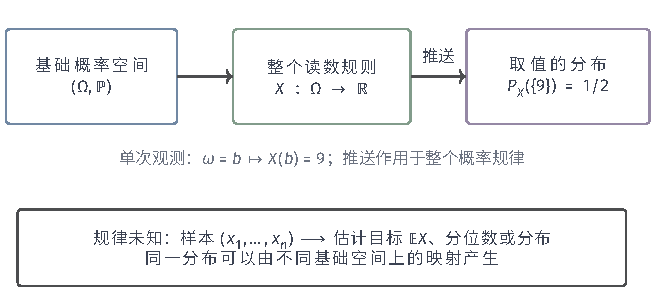
\includegraphics[width=\linewidth]{figures/02-mathematical-preliminaries-lower/01-random-variables-distributions-and-causality/tikz/rv-objects/figure.pdf}
  \caption{基础结果经随机变量映射成为读数；把事件概率推送到取值空间得到分布。分布未知时，样本用于估计指定目标，并不能唯一还原基础空间上的映射。}
\label{fig:rv-objects}
\end{figure}

\section{单个概率分布的描述}
\label{sec:rv-single-distribution}
前例中，不同设备状态可以得到同一个读数。若只关心读数，就把产生同一类读数的全部基础结果合在一起计算概率。设\(X\)取实值，它的分布测度记作\(\mathbb P_X\)，定义为
\[
 \mathbb P_X(B)=\mathbb P(X\in B)
 =\mathbb P\bigl(\{\omega:X(\omega)\in B\}\bigr),
 \qquad B\in\mathcal B(\mathbb R).
\]
这里\(B\)是读数空间中的集合，括号内的原像才是基础样本空间中的事件。\(\mathbb P\)给基础事件赋概率，\(\mathbb P_X\)给读数事件赋概率；等式说明二者怎样对应。随机变量\(X\)在取值空间上诱导的这个概率测度，称为它的\term{分布}（distribution）。

完整分布可以计算每个可测读数范围的概率。若当前只需要平均值或波动，可以先提取数值特征；若需要保留完整规律，则可用分布函数、相对于参考测度的密度，或积分变换来表示。为使后面的变换定义可直接使用，先建立期望。以下仍用\(F_X(x)=\mathbb P_X(({-\infty},x])\)表示累积到阈值\(x\)的概率，分布函数的性质在第~\ref{sec:rv-distribution}节说明。

\subsection{分布的数值特征}
\label{sec:rv-features}

完整分布能回答所有可测取值事件的概率，但一次计算往往只需要一个平均或波动尺度：报告一批读数的期望温度时，不必把整条分布列出来，只要一个数。数值特征通过对分布积分提取这些量。取值很大的地方可能只占很小的概率，所以定义平均之前，要核对相应的积分确实存在。
\label{sec:probability-expectation-conditional-expectation}
\paragraph{期望与均值}
% Baseline P:105-132
对非负随机变量\(X\)，定义
\[ \mathbb{E}[X]
  =\int_{\Omega}X(\omega)\,\mathrm{d}\mathbb{P}(\omega). \]
对一般实随机变量，写\(X=X^+-X^-\)。当
\(\mathbb{E}[|X|]<\infty\)时，正负两部分积分都有限，此时称\(X\)可积，并定义
\(\mathbb{E}[X]=\mathbb{E}[X^+]-\mathbb{E}[X^-]\)。不要求可积便随意相减\(\infty-\infty\)没有意义。

期望只依赖\(X\)的分布。对可测函数\(g\)，只要\(g(X)\)非负或可积，就有
\begin{equation}
  \mathbb{E}[g(X)]
  =
  \int_{\mathbb{R}}g(x)\,\mathrm{d}\mathbb{P}_X(x).
  \label{eq:probability-lotus}
\end{equation}
离散时，记\(p_X(x)=\mathbb P(X=x)\)，右侧是\(\sum_x g(x)p_X(x)\)；若分布具有密度\(f_X\)，即\(\mathbb P_X(B)=\int_B f_X(x)\,\mathrm dx\)，右侧则是\(\int g(x)f_X(x)\,\mathrm{d}x\)。这条“无须先求\(g(X)\)分布”的积分公式，会反复用于矩、蒙特卡洛估计和分布变换。

式~\eqref{eq:probability-lotus}直接来自推送测度的定义。对指示函数
\(g=\mathbb{I}_B\)，等式两侧分别为
\(\mathbb{P}(X\in B)\)与\(\mathbb{P}_X(B)\)，所以相等。线性性把结论推广到非负简单函数；任取递增到非负可测\(g\)的简单函数列，再在两侧使用单调收敛定理，即得非负情形。可积实值函数则分别对\(g^+\)和\(g^-\)应用这一结论。这个证明同时说明，等式并不要求\(X\)有密度。

\begin{example}[带噪观测的平均目标]
\label{ex:probability-noisy-observation}
设未知信号为\(\theta\)，观测为
\[ Y=\theta+\varepsilon,
  \qquad\mathbb{E}[\varepsilon]=0. \]
只要\(\varepsilon\)可积，就有\(\mathbb{E}[Y]=\theta\)。这并未说明一次读数接近
\(\theta\)，也未说明多个读数的平均必然收敛；后者还需要抽样依赖关系和矩条件。概率模型先把目标写成分布下的平均，后续误差结论再回答有限观测能否逼近这个平均。
\end{example}
\paragraph{方差与标准差}
% Baseline P:419-422
可积随机变量的均值记作\(\mu_X=\mathbb{E}[X]\)。若\(\mathbb{E}[X^2]<\infty\)，其方差为
\[ \operatorname{Var}(X)
  =\mathbb{E}\bigl[(X-\mu_X)^2\bigr]=\mathbb{E}[X^2]-\mu_X^2. \]
方差的非负平方根称为标准差，与原读数具有相同的计量单位。
% Baseline P:832-853

均值和方差便于计算，却不足以区分许多分布。若关心偏斜、尾部或独立和的分布变化，需要在这两个摘要之外保留信息：高阶矩增加摘要阶数；后面的积分变换还会把一系列摘要组织到一个函数中。

\paragraph{分位数}
% Baseline T:953-962
若给定累积概率水平\(q\in(0,1)\)，我们可以反过来寻找使累积概率达到或超过\(q\)的最小取值阈值。
\term{\(q\)分位数}（quantile）可定义为
\[
  F^{-1}(q)=\inf\{y:F(y)\geq q\},\qquad 0<q<1.
\]
这个广义逆为给定的\(F\)和\(q\)选出唯一的下分位数。更一般地，所有满足分位数
不等式的点组成集合
\[
  \mathcal Q_q=\{a:F(a^-)\leq q\leq F(a)\}.
\]
当\(F\)在水平\(q\)上存在平坦区间时，这个集合可能包含多个点；上述广义逆约定选取其中的下端代表。

\paragraph{高阶矩、偏度与峰度}
对正整数\(k\)，若\(\mathbb{E}[|X|^k]<\infty\)，则\(\mathbb{E}[X^k]\)称为\(k\)阶原点矩，
\(\mathbb{E}[(X-\mathbb{E}X)^k]\)称为\(k\)阶中心矩。三、四阶中心矩分别记录不对称性和大幅偏离均值的影响，但也随计量尺度改变。方差\(\sigma^2>0\)时，以\(\sigma^3\)和\(\sigma^4\)分别归一化，才得到偏度和峰度。有限低阶矩通常不能唯一确定分布。

\subsection{概率分布的表示}
\label{sec:rv-distribution}
数值特征只回答某一类查询。若要保留整个分布，可以记录全部阈值概率，也可以在参考测度下记录密度，或对一族指数函数积分。三种表示中的对象不同，存在条件也不同。

\subsubsection{基于分布函数的表示}
对实随机变量，分布函数为
\[ F_X(x)=\mathbb P_X(({-\infty},x])=\mathbb P(X\leq x). \]
它把一个概率测度写成一条关于阈值的函数。对\(a<b\)，半无限区间的差给出
\[ \mathbb P_X((a,b])=F_X(b)-F_X(a). \]
因此，知道全部\(F_X(x)\)就知道各半开区间的概率。由于这些区间生成实数轴的Borel事件族，分布函数唯一确定实数轴上的分布测度。

分布函数单调不减、右连续，且两端极限为
\[
  \lim_{x\to-\infty}F_X(x)=0,\qquad
  \lim_{x\to\infty}F_X(x)=1.
\]
反过来，每个具有这些性质的函数都对应某个实随机变量的分布。这是分布函数与分布测度之间的对应，不要求存在概率密度。

\subsubsection{基于参考测度的密度表示}
\label{sec:probability-radon-nikodym-change-measure}
若\(\mathbb{P}_X\)集中在可数点集上，可写成概率质量函数\(p_X(x)=\mathbb{P}(X=x)\)。若它相对于Lebesgue测度有密度\(f_X\)，则
\[ \mathbb{P}(X\in B)=\int_B f_X(x)\,\mathrm{d}x,
  \qquad F_X(x)=\int_{-\infty}^{x}f_X(t)\,\mathrm{d}t. \]
密度值不是单点概率。具有Lebesgue密度的分布满足\(\mathbb{P}(X=x)=0\)，但
\(f_X(x)\)仍可为正；在密度连续的点，它等于小邻域概率除以邻域长度后的局部极限；一般密度只在几乎处处意义下确定，不能在任意指定点都作这样的解释。
例如\(X\)在区间\([0,1/4]\)上均匀分布时，\(f_X(x)=4\mathbb{I}\{0\leq x\leq1/4\}\)。
密度值\(4\)可以大于\(1\)，因为概率由面积而非高度给出：
\(\mathbb{P}(0.10\leq X\leq0.15)=4\times0.05=0.2\)，而每个单点的概率仍为\(0\)。

图~\ref{fig:probability-density-cdf}把这一区分放在同一个分布上：密度图中的矩形面积，正是分布函数在区间两端的增量。因而从分布函数求区间概率不需要把连续结果变成单点概率。

\begin{figure*}[htbp]
  \centering
  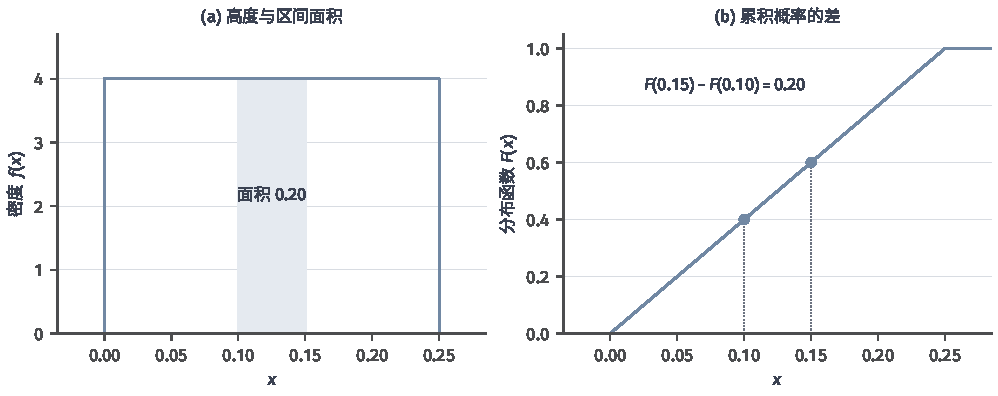
\includegraphics[width=\linewidth]{figures/02-mathematical-preliminaries-lower/01-random-variables-distributions-and-causality/matplotlib/probability-density-cdf/figure.pdf}
  \caption{区间\([0,1/4]\)上的均匀分布（解析式教学图）。左图阴影为\([0.10,0.15]\)的概率\(0.20\)，密度高度为\(4\)；右图的概率是\(F(0.15)-F(0.10)\)，两个端点本身均没有正概率质量。}
  \label{fig:probability-density-cdf}
\end{figure*}

在第~\ref{sec:probability-spaces-random-variables}节的四状态例子中，若把基础概率依次改成
\((0.1,0.2,0.3,0.4)\)，读数规则及取值范围都不变，但
\(\mathbb P(X=9)\)从\(1/2\)变成\(0.3\)。所以“能取哪些值”和“以什么概率取值”是两个问题。离散质量是相对于计数测度的密度；连续密度通常相对于Lebesgue测度，密度的数值不能脱离参考测度解释。
% Baseline P:136-246

离散的概率表与连续的密度函数，其实都是把分布写成某个参考测度下的权重：离散时参照计数测度，连续时通常参照Lebesgue测度。这引出一个统一的问题：在什么条件下，一个测度能写成另一个测度乘以某个权重，又怎样求出这个权重？
绝对连续先排除参考测度完全看不到的正质量区域，Radon--Nikodym导数在这一前提下给出权重；换测度时复用同一个权重，就不必为每种分布重新推导积分。

\paragraph{绝对连续与零集兼容性}
先考虑同一有限结果集合\(\Omega=\{\omega_1,\ldots,\omega_m\}\)上的两种概率分布\(P\)与\(Q\)。
记\(p_j=P(\{\omega_j\})\)、\(q_j=Q(\{\omega_j\})\)，则\((p_j)\)与\((q_j)\)就是两张概率表：各自列出每个结果出现的概率。
所谓“逐项比较”，就是固定同一个结果\(\omega_j\)，比较它在\(P\)下的概率\(p_j\)与在\(Q\)下的概率\(q_j\)。

例如，结果只有\(a,b,c\)三种，按这个顺序排列的概率表为
\[
  (p_1,p_2,p_3)=\left(\frac12,\frac14,\frac14\right),
  \qquad
  (q_1,q_2,q_3)=\left(\frac14,\frac14,\frac12\right).
\]
结果\(c\)在\(Q\)下出现的概率是在\(P\)下的两倍，\(a\)的概率则减半，\(b\)的概率不变。
若想用\(P\)下的样本估计\(Q\)下某个读数\(g\)的平均值，就应分别把\(a,b,c\)样本的读数乘以\(1/2,1,2\)，再对加权后的读数取样本平均。
这些权重正是\(q_j/p_j\)：在概率加权求和时，\(p_j\)乘以该比值就变成\(q_j\)，从而得到
\[
  \sum_{j=1}^{3}p_j\frac{q_j}{p_j}g(\omega_j)
  =\sum_{j=1}^{3}q_jg(\omega_j),
  \qquad (\omega_1,\omega_2,\omega_3)=(a,b,c).
\]
这里\(g\)是给每个结果指定一个实数读数的函数，右侧就是\(Q\)下的平均值。

上述例子中各个\(p_j\)均为正，概率比都有定义。但在一般的有限概率表中，若\(p_j=0\)而\(q_j>0\)，
\(P\)下的样本以概率\(1\)不会包含第\(j\)个结果，给已有样本重新加权也无法恢复\(Q\)分配给该结果的正概率。
例如，仍按\(a,b,c\)的顺序，改取
\[
  (p_1,p_2,p_3)=\left(\frac12,\frac12,0\right),
  \qquad
  (q_1,q_2,q_3)=\left(\frac14,\frac14,\frac12\right).
\]
从\(P\)抽样只能得到\(a\)和\(b\)，而\(Q\)给\(c\)分配了\(1/2\)的概率。
无论怎样调整\(a,b\)样本的权重，都不会产生\(c\)的贡献；即使给\(c\)指定任意有限权重\(w_c\)，其加权概率仍为
\[
  P(\{c\})w_c=0\times w_c=0,
\]
无法变成\(Q(\{c\})=1/2\)。所谓“无法补回这部分质量”，指的就是无法通过重加权恢复这\(1/2\)的概率。
若把读数取为\(g(\omega)=\mathbb{I}\{\omega=c\}\)，即只在结果为\(c\)时记为\(1\)、其余记为\(0\)，那么\(P\)样本的加权平均仍为\(0\)，而\(Q\)下的平均值为\(1/2\)。

图~\ref{fig:probability-zero-support-gap}把这一障碍画成两张概率表：\(a,b\)上的柱高可以经权重改变，\(c\)上为零的参考质量却没有可重加权的贡献。需要检查的是目标分布是否把正质量放在参考分布的零集上，而不是两组柱高是否接近。

\begin{figure}[htbp]
  \centering
  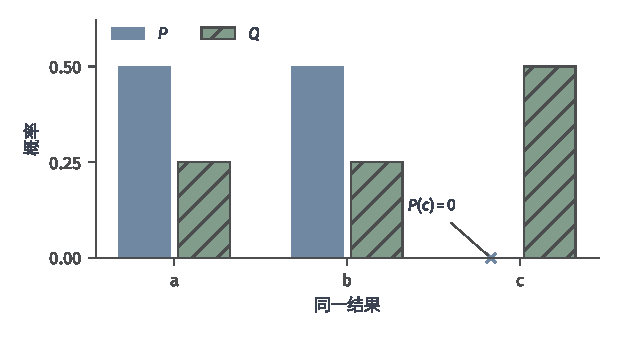
\includegraphics[width=105mm]{figures/02-mathematical-preliminaries-lower/01-random-variables-distributions-and-causality/matplotlib/probability-zero-support-gap/figure.pdf}
  \caption{参考分布缺少目标质量的三结果构造。蓝色实柱为\(P=(1/2,1/2,0)\)，绿色斜线柱为\(Q=(1/4,1/4,1/2)\)；叉号标出\(P(c)=0\)。任意有限权重仍给出\(P(c)w_c=0\)，不能恢复\(Q(c)=1/2\)。}
  \label{fig:probability-zero-support-gap}
\end{figure}

因此，若希望通过给\(P\)下的样本加权来计算\(Q\)下任意有界读数的平均，至少必须排除刚才的障碍：对每个结果\(\omega_j\)，只要\(P(\{\omega_j\})=0\)，就必须有\(Q(\{\omega_j\})=0\)。
这要求目标分布不给参考分布中概率为零的结果分配正概率。在有限结果集合上，检查所有单点就足够，因为任意事件的概率都是其中各个单点概率的和。

但在一般空间中，仅检查单点不够。例如，令\(P\)为\([0,1]\)上的均匀分布，\(Q\)为\([2,3]\)上的均匀分布。
两者对每个单点都给出零概率，却对事件\(A=[2,3]\)分别给出\(P(A)=0\)和\(Q(A)=1\)。
从\(P\)抽样无法得到落在\(A\)中的样本，给样本加权也无法恢复\(Q\)赋给\(A\)的概率。
所以，刚才的要求必须推广到每一个可测集合：
\[
  P(A)=0\Longrightarrow Q(A)=0,
  \qquad\text{对所有 }A\in\mathcal F\text{成立}.
\]
满足这一条件，就称\(Q\)对\(P\)绝对连续，记作\(Q\ll P\)。它把“参考分布中零概率的事件，在目标分布中也必须是零概率事件”写成了可检查的条件。

后面不仅要比较两个概率分布，还要讨论相对于计数测度、Lebesgue测度等参考测度的权重表示，因此把同一条件写成一般测度的定义。其中\(\mu\)对应参考测度，\(\nu\)对应希望表示的目标测度。
\begin{definition}[测度的绝对连续]
\label{def:probability-absolute-continuity}
设\(\nu\)与\(\mu\)为同一可测空间\((\Omega,\mathcal{F})\)上的测度。若
\[ \mu(A)=0\Longrightarrow\nu(A)=0,
  \qquad\text{对所有 }A\in\mathcal{F}\text{成立}, \]
则称\(\nu\)对\(\mu\)\term{绝对连续}（absolute continuity），记作\(\nu\ll\mu\)。
\end{definition}
它只要求\(\mu\)的零集也是\(\nu\)的零集，并不表示\(\nu(A)\leq\mu(A)\)，
也不自动提供有界的密度比。
这个定义先给出加权表示必须满足的零集条件，还没有构造权重函数。
接下来的有限分割计算先说明权重怎样由测度比得到；随后Radon--Nikodym定理再证明，在\(\sigma\)有限条件下，绝对连续足以保证一般空间中这样的权重函数存在。

\paragraph{有限分割上的密度表示}
先设\(\mu\)与\(\nu\)为有限测度，取有限可测分割
\(\Omega=A_1\mathbin{\dot\cup}\cdots\mathbin{\dot\cup}A_m\)，并假设\(\nu\ll\mu\)。
对\(\mu(A_j)>0\)的分块定义
\[ r(\omega)=\frac{\nu(A_j)}{\mu(A_j)},
  \qquad \omega\in A_j; \]
在\(\mu(A_j)=0\)的分块上令\(r=0\)。绝对连续性保证后一类分块也满足\(\nu(A_j)=0\)。因此，对任意由这些分块组成的事件\(A\)，
\[ \nu(A)=\int_A r\,\mathrm{d}\mu. \]
对在各分块上取有限实常数的函数\(g\)，逐项相加还给出
\begin{equation}
  \int_{\Omega}g\,\mathrm{d}\nu
  =
  \int_{\Omega}gr\,\mathrm{d}\mu.
  \label{eq:probability-finite-change-measure}
\end{equation}
一般定理要做的事，是在没有预先给定有限分块时构造同样的\(r\)\scite{math-kallenberg2021probability}。

\paragraph{一般测度的密度表示}
\begin{theorem}[Radon--Nikodym定理]
\label{thm:probability-radon-nikodym}
设\(\mu\)与\(\nu\)是\((\Omega,\mathcal{F})\)上的\(\sigma\)有限测度，且
\(\nu\ll\mu\)。则存在非负可测函数\(r\)，使每个\(A\in\mathcal{F}\)都满足
\begin{equation}
  \nu(A)=\int_A r\,\mathrm{d}\mu.
  \label{eq:probability-rn-representation}
\end{equation}
函数\(r\)在\(\mu\)-几乎处处意义下唯一，记为\(r=\mathrm{d}\nu/\mathrm{d}\mu\)，称为\term{Radon--Nikodym导数}
（Radon--Nikodym derivative）。
\end{theorem}

\begin{proof}
先设\(\mu,\nu\)有限，并令\(\lambda=\mu+\nu\)。在实线性空间
\(L^2(\lambda)\)上定义
\[
  T(f)=\int f\,\mathrm{d}\nu.
\]
由于\(\nu\leq\lambda\)，Cauchy--Schwarz不等式给出
\[
  |T(f)|
  \leq\int|f|\,\mathrm{d}\nu
  \leq\nu(\Omega)^{1/2}
       \left(\int f^2\,\mathrm{d}\nu\right)^{1/2}
  \leq\nu(\Omega)^{1/2}\lVert f\rVert_{L^2(\lambda)}.
\]
因此\(T\)是有界线性泛函。在完备内积空间中，有界线性泛函可以表示为与某个固定向量的内积。
\(L^2(\lambda)\)具有这一结构，所以存在
\(g\in L^2(\lambda)\)，使
\[
  \int f\,\mathrm{d}\nu=\int fg\,\mathrm{d}\lambda,
  \qquad f\in L^2(\lambda).
\]
这里用固定函数\(g\)表示测度\(\nu\)的积分，以便继续构造相对于\(\mu\)的密度；所用的Riesz表示性质可参考
\BookChapterRef{chap:functional-analysis-and-approximation}{卷1《数学准备：计算、分析与几何》的“函数空间”章}。
取\(f=\mathbb{I}_A\)可得\(\nu(A)=\int_Ag\,\mathrm{d}\lambda\)。若
\(A=\{g<0\}\)具有正测度，则对集合\(\{g\leq-1/k\}\)取指示函数会得到
\(\nu(\{g\leq-1/k\})<0\)的矛盾，故\(g\geq0\)几乎处处。又因为
\(\mu(A)=\lambda(A)-\nu(A)=\int_A(1-g)\,\mathrm{d}\lambda\geq0\)，同理有
\(g\leq1\)几乎处处。

令\(C=\{g=1\}\)。在\(C\)上有
\(\mu(C)=\int_C(1-g)\,\mathrm{d}\lambda=0\)，而\(\nu\ll\mu\)推出
\(\nu(C)=0\)。另一方面，\(\nu(C)=\int_Cg\,\mathrm{d}\lambda=\lambda(C)\)，所以
\(\lambda(C)=0\)。于是可以在其余部分定义
\[
  r=\frac{g}{1-g},
\]
并在\(C\)上任取值。由
\(\mathrm{d}\mu=(1-g)\,\mathrm{d}\lambda\)，对每个\(A\in\mathcal{F}\)都有
\[
  \int_A r\,\mathrm{d}\mu
  =\int_A\frac{g}{1-g}(1-g)\,\mathrm{d}\lambda
  =\int_Ag\,\mathrm{d}\lambda
  =\nu(A).
\]

若\(r_1,r_2\)都满足该表示，则对
\(A_k=\{r_1\geq r_2+1/k\}\)有
\[
  0=\int_{A_k}(r_1-r_2)\,\mathrm{d}\mu
  \geq\frac{1}{k}\mu(A_k),
\]
故\(\mu(A_k)=0\)。对\(k\)取并集得到\(r_1\leq r_2\)几乎处处；交换二者即得唯一性。

对\(\sigma\)有限的\(\mu,\nu\)，分别取有限测度覆盖并求交，可以把\(\Omega\)写成可数个互不相交、在两种测度下均有限的可测分块。在每个分块上使用上述构造，再把各块导数拼接，便得到全空间上的\(r\)。拼接后的表示可先对有限个分块验证，再由单调收敛推广到全部分块。
\end{proof}

这个证明先让\(\lambda=\mu+\nu\)同时支配两种测度，再把测度\(\nu\)表示为
\(L^2(\lambda)\)中的函数\(g\)。绝对连续性只用于排除\(g=1\)承载正质量，保证比值
\(g/(1-g)\)能够成为相对于\(\mu\)的密度。构造得到的是可测密度，并没有得到逐点上界。

\subsubsection{基于积分变换的表示}
\label{sec:probability-moment-transforms}
\paragraph{矩母函数与累积量生成函数}
逐个列出高阶矩，不便处理独立累计量。指数函数有一个方便的性质：它的幂级数把各阶幂放进同一个表达式；在允许交换求导与期望时，对参数求导便能取回相应的矩。对独立变量，和的指数矩又分解为各自指数矩的乘积，取对数就把这种乘积变成加法，因此同一构造还适合研究累计和。定义中的有限邻域用于保证这些运算有可用的起点。
\begin{definition}[矩母函数与累积量生成函数]
  \label{def:probability-moment-generating-functions}
设\(X\)为实随机变量。若存在\(\delta>0\)，使\(\mathbb E e^{tX}<\infty\)对全部\(|t|<\delta\)成立，则在该邻域上定义\term{矩母函数}（moment-generating function, MGF）为
\[ M_X(t)=\mathbb{E}[e^{tX}]. \]
\term{累积量生成函数}（cumulant-generating function）是
\[ K_X(t)=\log M_X(t). \]
\end{definition}
若可在积分号下求导，则\(M_X^{(k)}(0)=\mathbb{E}[X^k]\)。
矩存在却不保证矩母函数在原点邻域有限。取密度为
\(e^{-z^2/2}/\sqrt{2\pi}\)的标准高斯变量\(Z\)，令\(X=e^Z\)；
这样得到的正随机变量称为对数正态变量（lognormal random variable）。
对每个正整数\(k\)，配方得到
\[
 \mathbb E X^k
 =\frac1{\sqrt{2\pi}}\int_{\mathbb R}e^{kz-z^2/2}\,\mathrm dz
 =e^{k^2/2}<\infty.
\]
但对任意\(t>0\)，指数矩的被积函数是
\(e^{te^z-z^2/2}/\sqrt{2\pi}\)。当\(z\to+\infty\)时，\(e^z\)的增长压过\(z^2\)，
该被积函数最终大于\(1\)，所以在正半轴上的积分发散。
因此\(\mathbb E e^{tX}=\infty\)，虽有全部正整数阶矩，仍不满足上述邻域条件。

矩母函数满足上述有限邻域条件时，累积量生成函数的前两阶导数分别给出均值和方差。对随机向量\(\bm{X}\)，若联合指数矩在零向量的某个开邻域内有限，则定义
\[ K_{\bm{X}}(\bm{t})
  =\log\mathbb{E}\bigl[e^{\bm{t}^{\top}\bm{X}}\bigr], \]
混合偏导数给出联合累积量。独立变量的变换函数乘积及累积量可加法则在第~\ref{sec:rv-combinations}节说明。

% Baseline P:856-870
前两阶关系可以直接核对。若存在\(\delta>0\)，使
\(\mathbb E e^{tX}<\infty\)对全部\(|t|<\delta\)成立，取\(0<\delta_1<\delta_2<\delta\)。对\(|t|\leq\delta_1\)及\(j=1,2\)，存在有限常数\(C_j\)，使
\[ |X|^j e^{tX}\leq C_j\bigl(e^{\delta_2X}+e^{-\delta_2X}\bigr). \]
右侧可积，且不随\(t\)变化，因而允许在积分下求导，得到
\[
  M_X'(t)=\mathbb{E}[Xe^{tX}],\qquad
  M_X''(t)=\mathbb{E}[X^2e^{tX}].
\]
因为\(M_X(0)=1\)，
\[
  K_X'(0)=\frac{M_X'(0)}{M_X(0)}=\mathbb{E}X,
  \qquad
  K_X''(0)
  =M_X''(0)-M_X'(0)^2
  =\operatorname{Var}(X).
\]
矩母函数可能在零点的任何双侧邻域都不有限。研究分布极限时，需要一个对所有实参数都存在的变换。
\paragraph{特征函数与分布唯一性}
% Baseline P:875-878
\begin{definition}[特征函数]
  \label{def:probability-characteristic-function}
实随机变量\(X\)的特征函数为\(\varphi_X(t)=\mathbb E e^{\mathrm i tX}\)，其中\(t\in\mathbb R\)。随机向量的版本为\(\varphi_{\bm X}(\bm t)=\mathbb E e^{\mathrm i\bm t^\top\bm X}\)。复数期望分别对实部与虚部积分。
\end{definition}
由于复指数的绝对值恒为\(1\)，特征函数总存在。它用振荡而非指数放大取值，因此与可能发散的矩母函数承担不同职责；后面将用它把独立和的分布极限转成函数的逐点极限。

变换还有一个有限低阶矩所没有的性质：保留完整的特征函数，就保留了分布。
\begin{theorem}[变换函数的分布唯一性]
\label{thm:rv-transform-uniqueness}
同维随机向量的特征函数在所有实向量参数上相同，当且仅当它们的分布相同。
若两个矩母函数都在原点的某个共同开邻域内有限，并在该邻域内相同，
它们也确定相同的分布。
\end{theorem}
这里引用概率变换的唯一性定理，不展开所需的Fourier反演论证\scite{math-kallenberg2021probability}。
它把“两个变换相同”转成“两个分布相同”；只比较有限个矩或有限个参数点，
没有这种唯一性保证。

\section{随机变量的联合、条件与独立关系}
\label{sec:rv-relations}
两台设备即使各自具有相同误差分布，共同偏高与一高一低仍会给出不同的平均结果。下面先建立联合规律和独立性，再说明已知一项读数后怎样更新另一项的描述。

\subsection{随机变量的联合关系}
\label{sec:rv-joint}
\label{sec:probability-joint-marginal-conditional}
\subsubsection{联合分布与边缘分布}
% Baseline P:312-333
随机向量\((X,Y)\)的联合分布是映射\(\omega\mapsto(X(\omega),Y(\omega))\)在乘积空间上诱导的概率测度。离散情形中，
联合质量\(p_{X,Y}(x,y)\)给出完整表格，边缘分布由求和消去另一坐标：
\[ p_X(x)=\sum_y p_{X,Y}(x,y),
  \qquad p_Y(y)=\sum_x p_{X,Y}(x,y). \]
若联合分布有密度，则相应运算变为
\[ f_X(x)=\int f_{X,Y}(x,y)\,\mathrm{d}y. \]
一般情形不需要质量函数或密度。记坐标投影为\(\pi_X(x,y)=x\)，则边缘分布就是联合分布经\(\pi_X\)的推送：
\[
  \mathbb{P}_X(A)
  =\mathbb{P}_{(X,Y)}(A\times\mathcal{Y}).
\]
对非负可测函数\(g\)，式~\eqref{eq:probability-lotus}给出
\[
  \int g(x)\,\mathbb{P}_X(\mathrm{d}x)
  =
  \int g\bigl(\pi_X(x,y)\bigr)\,
       \mathbb{P}_{(X,Y)}(\mathrm{d}x,\mathrm{d}y).
\]
若联合分布有密度，再对右侧使用Tonelli定理，才得到对\(y\)积分的边缘密度公式。因而“边缘化”首先是测度推送，求和或积分只是它在特定参考测度下的表达。

边缘化会丢掉变量如何共同变化的信息。两个不同联合分布可以拥有完全相同的两个边缘分布：只看各自边缘，看不出两个读数是一起升高、彼此独立还是总朝相反方向变化。下面用一个只取两个值的例子把这一丢失演示出来。

\subsubsection{协方差与相关系数}
% Baseline P:423-430
已知两个边缘方差，还不能判断合成读数的波动。将各读数减去自身均值后再相乘，就可把同向偏离与反向偏离区分开；把这些乘积按联合规律平均，得到进入和的方差公式的交叉项。这个量只保留二阶共同变化，不能代替完整联合分布。
对二阶可积的\(X,Y\)，协方差为
\[ \operatorname{Cov}(X,Y)
  =\mathbb{E}\bigl[(X-\mathbb{E}X)(Y-\mathbb{E}Y)\bigr]. \]
Cauchy--Schwarz不等式保证它有限。方差满足
\[ \operatorname{Var}(aX+b)=a^2\operatorname{Var}(X), \]
而
\[ \operatorname{Var}(X+Y)
  =\operatorname{Var}(X)+\operatorname{Var}(Y)+2\operatorname{Cov}(X,Y). \]
只有协方差为零时，方差才直接相加；独立是协方差为零的充分条件，但通常不是必要条件。

若各坐标二阶可积，随机向量的均值和协方差为
% Baseline P:1090-1098
\[ \bm{\mu}=\mathbb{E}\bm{X},
  \qquad\bm{\Sigma}=\mathbb{E}\bigl[(\bm{X}-\bm{\mu})(\bm{X}-\bm{\mu})^{\top}\bigr]. \]
对任意\(\bm{u}\in\mathbb{R}^d\)，
\[
  \bm{u}^{\top}\bm{\Sigma}\bm{u}
  =\mathbb{E}\left[
    \bigl(\bm{u}^{\top}(\bm{X}-\bm{\mu})\bigr)^2
  \right]\geq0,
\]
所以协方差矩阵总是对称半正定。

若两个变量的方差都为正，相关系数定义为
\[ \rho_{X,Y}=\frac{\operatorname{Cov}(X,Y)}{\sqrt{\operatorname{Var}(X)\operatorname{Var}(Y)}}. \]
Cauchy--Schwarz不等式给出\(|\rho_{X,Y}|\leq1\)。零方差变量是几乎处处常数，不应代入分母为零的相关系数公式。
把读数转换成二元误差标记\(U,V\in\{0,1\}\)。令两个标记各自以概率\(1/2\)取零或一，即固定边缘规律为
\[
U\sim\operatorname{Bernoulli}(1/2),\qquad
V\sim\operatorname{Bernoulli}(1/2).
\]
图~\ref{fig:rv-dependence}中的联合质量仍可给出三种不同的平均效果：
\[
\begin{array}{c|ccc}
 & V=U & U,V\text{独立} & V=1-U\\ \hline
\operatorname{Cov}(U,V)&1/4&0&-1/4\\
\mathbb P(U+V=0)&1/2&1/4&0\\
\mathbb P(U+V=1)&0&1/2&1\\
\mathbb P(U+V=2)&1/2&1/4&0
\end{array}
\]
\begin{figure}[htbp]
  \centering
  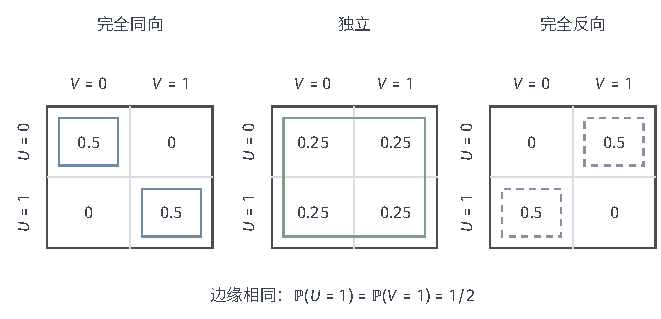
\includegraphics[width=\linewidth]{figures/02-mathematical-preliminaries-lower/01-random-variables-distributions-and-causality/tikz/rv-dependence/figure.pdf}
  \caption{边缘质量相同的三个联合分布。格内数字是联合概率，各行各列的和始终为\(1/2\)；质量的位置改变协方差及和的分布。}
\label{fig:rv-dependence}
\end{figure}

\begin{example}[区域分布的质心与主轴]
\label{ex:probability-region-moments}
设平面区域\(A\subset\mathbb R^2\)的面积\(|A|\)有限且非零，并有有限二阶矩。在\(A\)上按面积均匀抽取位置\(\bm X=(X_1,X_2)^\top\)，其均值与协方差为
\[
 \bm\mu=\frac1{|A|}\int_A\bm x\,\mathrm d\bm x,
 \qquad
 \bm\Sigma=\frac1{|A|}\int_A(\bm x-\bm\mu)(\bm x-\bm\mu)^\top\,\mathrm d\bm x.
\]
均值是区域的质心；单位方向\(\bm u\)上的位置方差为\(\bm u^\top\bm\Sigma\bm u\)。因此最大特征值的特征向量给出位置分散最大的主轴方向；最大特征值重复时，这个方向可能不唯一。图像区域的面积、质心与二阶矩可用同一分布语言表示，但这里均匀抽取的是位置，不是把像素灰度直接当作概率。
\end{example}

\subsection{随机变量的独立关系}
\label{sec:probability-moments-independence}
% Baseline P:720-821

联合规律可能由边缘规律直接相乘得到。此时，知道一项取什么值不会改变另一项的分布；这种关系称为独立性。先用事件概率描述它，再检查它与零协方差的区别。

\subsubsection{独立、不相关与非线性依赖}
若随机变量\(X,Y\)满足
\[ \mathbb{P}(X\in A,Y\in B)
  =\mathbb{P}(X\in A)\mathbb{P}(Y\in B) \]
对所有Borel集合\(A,B\)成立，就称二者\term{独立}（independent）。对非负可测函数\(g,h\)，独立性给出
\[
 \mathbb{E}[g(X)h(Y)]=\mathbb{E}[g(X)]\mathbb{E}[h(Y)],
\]
等式按非负扩展实数解释，并约定\(0\cdot\infty=0\)。对实值函数，若\(g(X)\)与\(h(Y)\)分别可积，则乘积也可积，且同一等式两侧均为有限值。
证明从指示函数开始：独立性正好说明结论对
\(g=\mathbb{I}_A\)、\(h=\mathbb{I}_B\)成立。线性性把它推广到非负简单函数，再分别对两个因子使用单调收敛，得到非负情形。
对分别可积的实值因子，先把非负结论用于\(|g|,|h|\)，得到乘积的绝对期望有限，再分解正负部分即可。
仅有乘积可积并不足够：一个因子恒为零时乘积可积，另一个因子的期望却可能不存在，不能据此写出右侧的有限期望乘积。

协方差只检查中心化变量的一次乘积。令\(X\)在\([-1,1]\)上均匀分布，并取\(Y=X^2\)。对称性给出
\[ \operatorname{Cov}(X,Y)
  =\mathbb{E}[X^3]-\mathbb{E}[X]\mathbb{E}[X^2]=0, \]
但\(Y\)由\(X\)完全决定；知道\(X\)便能确定\(Y\)，所以二者不独立。零协方差只排除了线性二阶关联。

\subsection{随机变量的条件关系}
看到第一台设备的读数后，第二台设备原来的边缘描述可能不再充分。若查询的是平均读数，可以把已见信息固定下来计算条件期望；若查询的是越界概率、分位数或下一次随机生成的规律，则需要条件分布。两项查询使用相同的信息，但要求保留的结果不同。

\subsubsection{条件信息下的均值关系}
\label{sec:rv-conditional-expectation}
% Baseline P:434-524
预测一个结果时，可用的信息往往不是结果本身，而只是一部分观察：可能知道一次测量落在哪个区间却不知道精确数值，也可能知道掷出的点数是奇数却不知道是几点。要把“知道一部分”写成可以计算的对象，需要先说清哪些事件能由这部分信息区分，再要求预测在每个可区分的事件上保持原有的平均。

有限情形可以直接说清。若手头的信息只把样本空间分成有限组\(A_1,\ldots,A_m\)，那么预测值在每组之内只能取同一个常数——超过了这些信息就没有依据；而要让这个常数不与已知信息冲突，取该组内\(X\)的平均是自然的选择。于是“只用已有信息”与“不改变各组平均”这两条要求，共同确定了预测值。表~\ref{tab:probability-finite-partition-predictions}给出可以逐项核对的例子。

连续取值时不能照搬“给定\(X=x\)”这一步。若\(P(X=x)=0\)，事件\(\{X=x\}\)的概率为零，比值
\(\mathbb E[X\mathbb I_{\{X=x\}}]/\mathbb P(X=x)\)成为\(0/0\)，没有定义；对每个\(x\)都零概率地单独处理，也无法拼出一个整体的答案。这正是需要换一种写法的原因。

出路是放弃逐点条件，改为整体要求：答案在每一个仅由\(X\)决定的事件上保持原来的平均。仅由\(X\)决定的事件正是\(\sigma(X)\)中的集合，因而条件用子\(\sigma\)代数表示，而不是用单个事件表示。下面先明确“由观察生成的信息”，再给出这一定义。

子\(\sigma\)代数\(\mathcal{G}\subseteq\mathcal{F}\)表示当前可用信息。预测值只能使用这些信息，并且在每个可以由当前信息区分的事件上保持原来的平均。
\begin{definition}[观测生成的信息]
  \label{def:probability-generated-information}
若\(X:\Omega\to(\mathcal X,\mathcal A)\)是随机变量，记
\(\sigma(X)=\{X^{-1}(A):A\in\mathcal A\}\)。它是使\(X\)可测的最小\(\sigma\)代数，表示仅观察\(X\)能够区分的事件。多个观测生成的信息是包含它们全部可测逆像的最小\(\sigma\)代数。
\end{definition}
例如只观察分组编号，就不能在同一组内区分两个原始结果。写\(\mathbb E[Y\mid X]\)时，真正限制答案的信息是\(\sigma(X)\)，不是单个零概率事件\(\{X=x\}\)。
\begin{definition}[条件期望]
  \label{def:probability-conditional-expectation}
对\(X\in L^1(\mathbb P)\)，\term{条件期望}（conditional expectation）
\(\mathbb{E}[X\mid\mathcal{G}]\)是满足下列两项条件的可积随机变量\(Z\)：
\[ Z\text{ 对 }\mathcal{G}\text{ 可测},
  \qquad\int_A Z\,\mathrm{d}\mathbb{P}=\int_A X\,\mathrm{d}\mathbb{P}\quad(A\in\mathcal{G}). \]
\end{definition}
第一项要求答案只能使用\(\mathcal{G}\)中的信息，第二项要求它在每个可由当前信息识别的事件上保留\(X\)的平均\scite{math-kallenberg2021probability}。在有限分组情形，第二项正是“每组内部平均值不变”，第一项正是“同组之内取同一个常数”；两条合起来就唯一确定了前面所说的逐组平均。

这里有一点容易忽略：条件期望本身是一个随机变量，不是常数。\(\mathbb E[X\mid\mathcal G]\)随\(\omega\)变化，但它只通过\(\mathcal G\)能够区分的部分变化——在同一组之内取值相同。所以它是“把已知信息作为输入的函数”，写成\(\mathbb E[X\mid X]\)等于\(X\)，写成\(\mathbb E[X\mid \{\varnothing,\Omega\}]\)则是常数\(\mathbb E X\)。已知的信息越多，\(\mathcal G\)越大，答案就越细致；两个极端分别是不用任何信息和已知全部信息。

\begin{theorem}[条件期望的存在与唯一性]
\label{thm:probability-conditional-expectation-existence}
若\(X\in L^1(\mathbb{P})\)，则\(\mathbb{E}[X\mid\mathcal{G}]\)存在，并在几乎处处意义下唯一。
\end{theorem}

\begin{proof}
先设\(X\geq0\)。在\((\Omega,\mathcal{G})\)上定义有限测度
\[ \nu(A)=\int_A X\,\mathrm{d}\mathbb{P}. \]
若\(\mathbb{P}(A)=0\)，则\(\nu(A)=0\)，所以\(\nu\ll\mathbb{P}|_{\mathcal{G}}\)。Radon--Nikodym定理给出非负、
\(\mathcal{G}\)-可测的\(Z\)，使\(\nu(A)=\int_A Z\,\mathrm{d}\mathbb{P}\)。对一般可积\(X\)，分别对
\(X^+\)与\(X^-\)使用这一构造并取差，即得存在性。

若\(Z_1,Z_2\)都满足定义，令\(D=Z_1-Z_2\)。对每个\(A\in\mathcal{G}\)，\(\int_A D\,\mathrm{d}\mathbb{P}=0\)。若
\(\mathbb{P}(D>0)>0\)，则某个集合\(A_k=\{D\geq1/k\}\)具有正概率，从而
\[ \int_{A_k}D\,\mathrm{d}\mathbb{P}
  \geq\frac{1}{k}\mathbb{P}(A_k)>0, \]
产生矛盾。因此\(D\leq0\)几乎处处。交换\(Z_1,Z_2\)可得\(D\geq0\)几乎处处，故二者几乎处处相等。
\end{proof}

积分的线性性与上述唯一性说明，条件期望也保持线性组合。
对非负变量，存在证明给出的Radon--Nikodym导数非负；
因此若\(X\leq Y\)且两者可积，对\(Y-X\)使用该构造便得到
\(\mathbb E[X\mid\mathcal G]\leq\mathbb E[Y\mid\mathcal G]\)几乎处处。
这就是条件期望的保序性。

若\(X\)本来就对\(\mathcal{G}\)可测，则\(\mathbb{E}[X\mid\mathcal{G}]=X\)几乎处处。若\(X\)与\(\mathcal{G}\)
独立，则条件期望等于常数\(\mathbb{E}[X]\)。若\(U\)有界且\(\mathcal{G}\)-可测，则
\begin{equation}
  \mathbb{E}[UX\mid\mathcal{G}]
  =
  U\mathbb{E}[X\mid\mathcal{G}].
  \label{eq:probability-taking-out-known-factor}
\end{equation}
可积的非有界\(U\)需要另外核对乘积可积性，不能仅凭“已知量可提出”略去条件。

有限分组把抽象定义化成逐组平均。若
\(A_1,\ldots,A_m\)是有限可测分割，
\(\mathcal{G}=\sigma(A_1,\ldots,A_m)\)，且每个
\(\mathbb{P}(A_j)>0\)，则
\begin{equation}
  \mathbb{E}[X\mid\mathcal{G}]
  =
  \sum_{j=1}^{m}
  \frac{\mathbb{E}[X\mathbb{I}_{A_j}]}
       {\mathbb{P}(A_j)}
  \mathbb{I}_{A_j}.
  \label{eq:probability-finite-partition-conditional-expectation}
\end{equation}
若某个分组概率为零，该组上的取值可以任意指定，因为条件期望只在几乎处处意义下唯一。

表~\ref{tab:probability-finite-partition-predictions}给出一个可复核例子。令
\(\mathcal{G}\)只能区分
\(A=\{\omega_1,\omega_2\}\)与
\(B=\{\omega_3,\omega_4\}\)。不使用分组信息时，最佳常数预测是
\(U_0=\mathbb{E}X=3.4\)；规则\(U_{\mathrm{grp}}\)虽然按组取值，却随意地在
\(A,B\)上分别预测\(0,4\)；条件均值\(m=\mathbb{E}[X\mid\mathcal{G}]\)则在两组
上分别等于\(1.2,5.6\)。
\begin{table}[htbp]
  \centering
  \small
  \begin{tabular}{ccccccc}
    \toprule
    结果 & 概率 & \(X\) & 分组 & \(U_0\) & \(U_{\mathrm{grp}}\) & \(m\) \\
    \midrule
    \(\omega_1\) & \(0.2\) & \(0\) & \(A\) & \(3.4\) & \(0\) & \(1.2\) \\
    \(\omega_2\) & \(0.3\) & \(2\) & \(A\) & \(3.4\) & \(0\) & \(1.2\) \\
    \(\omega_3\) & \(0.1\) & \(4\) & \(B\) & \(3.4\) & \(4\) & \(5.6\) \\
    \(\omega_4\) & \(0.4\) & \(6\) & \(B\) & \(3.4\) & \(4\) & \(5.6\) \\
    \midrule
    \multicolumn{4}{r}{平方风险\(\ \mathbb{E}[(X-U)^2]\)} &
    \(5.64\) & \(2.80\) & \(0.80\) \\
    \bottomrule
  \end{tabular}
  \caption{有限分组下的三类预测。分组信息使预测可以随\(A,B\)变化，但只有逐组条件
  均值在全部\(\mathcal{G}\)-可测平方可积预测中达到最小平方风险。}
  \label{tab:probability-finite-partition-predictions}
\end{table}
按定义核对\(m\)，只需在\(\mathcal{G}\)能区分的事件上验证第二条要求，即
\(A,B,\varnothing,\Omega\)。在\(A\)上，
\[
  \int_A X\,\mathrm{d}\mathbb{P}
  =0\times0.2+2\times0.3=0.6
  =\mathbb{P}(A)\times1.2
  =\int_A 1.2\,\mathrm{d}\mathbb{P},
\]
在\(B\)上同理有\(4\times0.1+6\times0.4=2.8=0.5\times5.6\)。而在\(\Omega\)上两者
都等于\(\mathbb E X=3.4\)，这正是全期望公式在两组情形下的表现。反过来，
\(U_{\mathrm{grp}}\)在\(A\)上取值\(0\)而组内平均为\(1.2\)，第二条要求不满足，
所以它不是条件期望。逐组平均之所以在这里唯一确定答案，是因为除两个分组外
\(\mathcal{G}\)不再含其他集合，核对任务只有这么几项；一般情形下可测性要求把范围
限制在\(\sigma(A_1,\ldots,A_m)\)中，结论仍然相同。

三列风险依次说明不同问题：获得分组信息可以优于无信息常数，但使用信息本身不保证已经
最优；式~\eqref{eq:probability-finite-partition-conditional-expectation}还要在每组
内选择正确的条件平均。三列中只有\(m\)同时满足两条定义条件，风险\(0.80\)也比另外两列低，
这两个事实不是巧合：\(\mathcal{G}\)-可测平方可积预测中使平方风险最小者，正是条件期望，
下面的平方分解会说明原因。
% Baseline P:532-625
\begin{theorem}[塔式性质]
\label{thm:probability-tower-property}
若\(X\in L^1\)，且\(\mathcal{H}\subseteq\mathcal{G}\subseteq\mathcal{F}\)，则
\[ \mathbb{E}\bigl[\mathbb{E}[X\mid\mathcal{G}]
  \mid\mathcal{H}\bigr]=\mathbb{E}[X\mid\mathcal{H}] \]
几乎处处成立。
\end{theorem}

\begin{proof}
左侧对\(\mathcal{H}\)可测。对任意\(A\in\mathcal{H}\)，由于\(A\in\mathcal{G}\)，条件期望定义给出
\[
  \int_A
  \mathbb{E}\bigl[\mathbb{E}[X\mid\mathcal{G}]
  \mid\mathcal{H}\bigr]\,\mathrm{d}\mathbb{P}
  =
  \int_A\mathbb{E}[X\mid\mathcal{G}]\,\mathrm{d}\mathbb{P}
  =
  \int_A X\,\mathrm{d}\mathbb{P}.
\]
左侧因而满足\(X\)关于\(\mathcal{H}\)的条件期望定义，唯一性给出结论。
\end{proof}

取\(\mathcal{H}=\{\varnothing,\Omega\}\)，便得到\term{全期望公式}（law of total expectation）
\begin{equation}
  \mathbb{E}\bigl[\mathbb{E}[X\mid\mathcal{G}]\bigr]
  =
  \mathbb{E}[X].
  \label{eq:probability-total-expectation}
\end{equation}
这说明条件化改变可用信息，却不改变再平均后的总体均值。

\paragraph{全方差分解}
设\(X\in L^2\)，记\(m=\mathbb{E}[X\mid\mathcal{G}]\)。分解
\[ X-\mathbb{E}X=(X-m)+(m-\mathbb{E}X). \]
在展开平方前，需要先确认条件均值仍然二阶可积。
对每个有理数\(q\)，条件期望的线性性与保序性给出
\[
 \mathbb E[X^2\mid\mathcal G]-2qm+q^2
 =\mathbb E[(X-q)^2\mid\mathcal G]\geq0.
\]
有理数只有可数个，可以在同一个满测集上同时使用这些不等式。
由于\(\sup_{q\in\mathbb Q}(2qm-q^2)=m^2\)，得到
\[
  |m|^2
  \leq
  \mathbb{E}[X^2\mid\mathcal{G}].
\]
再取期望并使用全期望公式，得到
\[
  \mathbb{E}[m^2]\leq\mathbb{E}[X^2]<\infty.
\]
因此\(m\in L^2\)，上面分解中的两项都二阶可积，其乘积由Cauchy--Schwarz不等式保证可积。又因为第二项对
\(\mathcal{G}\)可测，而\(\mathbb{E}[X-m\mid\mathcal{G}]=0\)，所以交叉项期望为
\[ \mathbb{E}\bigl[(X-m)(m-\mathbb{E}X)\bigr]
  =\mathbb{E}\left[(m-\mathbb{E}X)\mathbb{E}[X-m\mid\mathcal{G}]\right]=0. \]
展开平方得到\term{全方差公式}（law of total variance）
\begin{equation}
  \operatorname{Var}(X)
  =
  \mathbb{E}\bigl[\operatorname{Var}(X\mid\mathcal{G})\bigr]
  +
  \operatorname{Var}\bigl(\mathbb{E}[X\mid\mathcal{G}]\bigr),
  \label{eq:probability-total-variance}
\end{equation}
其中
\[ \operatorname{Var}(X\mid\mathcal{G})
  =\mathbb{E}\bigl[(X-m)^2\mid\mathcal{G}\bigr]. \]
第一项是获得\(\mathcal{G}\)后仍无法解释的平均波动，第二项是不同信息状态之间的可解释波动。

刚才的平方界是条件Jensen不等式（conditional Jensen inequality）的一个实例。
一般地，若\(\phi:\mathbb R\to\mathbb R\)为凸函数，\(X\)与\(\phi(X)\)都可积，则
\[
 \phi\bigl(\mathbb E[X\mid\mathcal G]\bigr)
 \leq\mathbb E[\phi(X)\mid\mathcal G]\quad\text{几乎处处}.
\]
其依据仍是仿射下界：在每个有理点选取一条支撑线
\(a_qx+b_q\leq\phi(x)\)，凸函数的连续性保证这些支撑线的上确界等于\(\phi\)。
对每条线取条件期望，得到
\(a_qm+b_q\leq\mathbb E[\phi(X)\mid\mathcal G]\)，
再在共同满测集上取可数上确界即可。
对有限维随机向量，把支撑线换成仿射支撑超平面，论证相同；
凸函数只定义在凸域上时，还需条件均值属于该域，并核对相关量的可积性。
取不含额外信息的平凡条件，便得到通常的积分Jensen不等式。

\paragraph{条件均值的平方损失最优性}
\begin{theorem}[条件均值的平方损失最优性]
\label{thm:probability-conditional-mean-l2-projection}
设\(X\in L^2(\mathbb{P})\)。在所有\(\mathcal{G}\)-可测且二阶可积的随机变量\(U\)中，
\[ m=\mathbb{E}[X\mid\mathcal{G}] \]
唯一地在几乎处处意义下最小化\(\mathbb{E}[(X-U)^2]\)。
\end{theorem}

\begin{proof}
\(L^2(\mathcal{G})\)是\(L^2(\mathcal{F})\)的闭线性子空间，上文直接证明的条件平方界已经说明
\(m\in L^2(\mathcal{G})\)。对每个\(U\in L^2(\mathcal{G})\)，Cauchy--Schwarz不等式保证
\((X-m)U\)可积，因而可以提出已知因子并使用塔式性质，得到
\[ \mathbb{E}[(X-m)U]
  =\mathbb{E}\left[U\mathbb{E}[X-m\mid\mathcal{G}]\right]=0. \]
所以\(X-m\)与整个\(L^2(\mathcal{G})\)正交，\(m\)就是\(X\)到该闭子空间的正交投影。直接展开
\begin{equation}
  \mathbb{E}[(X-U)^2]
  =
  \mathbb{E}[(X-m)^2]
  +
  \mathbb{E}[(m-U)^2],
  \label{eq:probability-pythagorean-prediction}
\end{equation}
交叉项因正交性消失。第二项非负，且仅当\(U=m\)几乎处处时为零。
\end{proof}

图~\ref{fig:probability-conditional-projection}把这一平方分解放在一个能画出的精确模型中。设基础结果只有两种，概率各为\(1/2\)，且可用信息不能区分它们。每个随机变量由它在两种结果上的取值表示为一个平面向量；允许的预测只能是常量，因此落在对角线\(U=(c,c)\)上。取\(X=(0,2)\)，其条件均值为\(m=(1,1)\)。若改用\(U=(2,2)\)，则\(X-m\)与\(m-U\)正交，平方风险从最小值\(1\)增加为\(1+1=2\)。这里的距离来自随机变量之间的\(L^2\)范数，图中的两个坐标不是两次抽样的时间顺序。一般条件信息可对应更高维的可测预测子空间，同一个正交分解仍由上面的证明给出。

\begin{figure}[htbp]
  \centering
  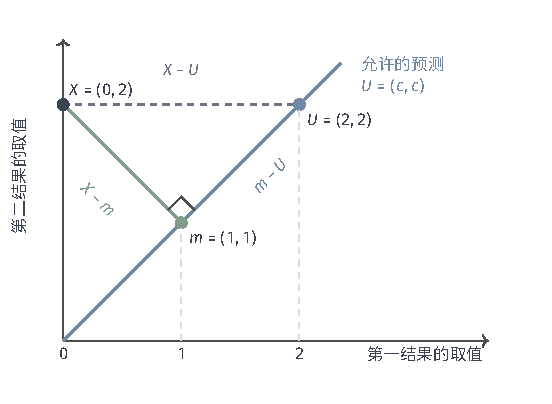
\includegraphics[width=92mm]{figures/02-mathematical-preliminaries-lower/01-random-variables-distributions-and-causality/tikz/probability-conditional-projection/source.pdf}
  \caption{两等概率结果上的条件均值投影。横纵坐标分别记录随机变量在两个基础结果上的取值；平凡信息下允许预测的集合是对角线。\(m\)是\(X\)在该线上的投影，直角标记对应误差正交。此例的\(L^2\)范数平方是图中欧氏长度平方的\(1/2\)，所以三边对应的平方风险满足\(2=1+1\)。}
  \label{fig:probability-conditional-projection}
\end{figure}

条件期望的存在只需要\(X\in L^1\)，这时它由Radon--Nikodym导数给出。“正交投影”和平方损失最优性则需要\(X\in L^2\)。若二阶矩无限，条件期望仍可能
存在，但不能直接套用上述\(L^2\)投影结论。

\subsubsection{条件信息下的分布关系}
\label{sec:rv-conditional-distribution}
% Baseline P:370-413
当条件变量连续时，事件\(\{X=x\}\)常有零概率，直接相除不再可行。需要把“每个条件值对应一个分布”组织成能继续积分的对象。
\begin{definition}[概率核]
  \label{def:probability-kernel}
  给定可测空间\((\mathcal X,\mathcal A)\)、\((\mathcal Y,\mathcal B)\)，\term{概率核}（probability kernel）是映射
  \[ K:\mathcal X\times\mathcal B\to[0,1], \]
  满足：对每个\(x\in\mathcal X\)，\(K(x,\cdot)\)是\((\mathcal Y,\mathcal B)\)上的概率测度；对每个\(B\in\mathcal B\)，\(x\mapsto K(x,B)\)是\(\mathcal A\)-可测函数。
\end{definition}
第一项保证每个条件值给出合法分布，
第二项保证再对\(X\)积分是合法运算。

可测并不等于连续。例如取在\([-1,1]\)上均匀分布的\(X\)，令\(Y=\mathbb I\{X\geq0\}\)，则\(K(x,\{1\})=\mathbb I\{x\geq0\}\)是合法概率核在事件\(\{1\}\)上的取值，却在\(x=0\)处跳变。条件值\(x\)可以连续取值，条件分布随\(x\)变化仍可不连续。

\begin{definition}[正则条件分布]
  \label{def:probability-regular-conditional-distribution}
若概率核\(K\)对所有\(A\in\mathcal A\)、\(B\in\mathcal B\)满足
\begin{equation}
  \mathbb{P}(X\in A,Y\in B)
  =
  \int_A K(x,B)\,\mathbb{P}_X(\mathrm{d}x),
  \label{eq:probability-regular-conditional-kernel}
\end{equation}
就把\(K(x,\cdot)\)称为\(Y\)给定\(X=x\)的一个\term{正则条件分布}（regular conditional distribution）。
\end{definition}
对每个固定可测集\(B\)，两个版本的\(K(x,B)\)在\(\mathbb P_X\)-几乎处处意义下相同；若\(\mathcal Y\)是下面的标准Borel空间，还可选取一个共同零测集，使其外的条件概率测度相同。零概率条件点上的取值通常不能由联合分布唯一决定。

\begin{example}[条件分布版本可以怎样不同]
\label{ex:probability-conditional-kernel-versions}
设\(X\sim\operatorname{Unif}[0,1]\)，并令\(Y=X\)。给定\(x\)，取
\(K(x,\cdot)=\delta_x\)，即全部条件概率质量集中在\(y=x\)。对任意Borel集\(A,B\)，
\[
 \begin{aligned}
 \mathbb P(X\in A,Y\in B)
 &=\mathbb P(X\in A\cap B)\\
 &=\int_A\mathbb I_B(x)\,\mathbb P_X(\mathrm dx)
  =\int_A K(x,B)\,\mathbb P_X(\mathrm dx).
 \end{aligned}
\]
因此\(K\)是一个正则条件分布。现在只在\(x=1/2\)处把\(\delta_x\)改成\(\delta_0\)，
其余点不变，得到另一个可测概率核\(\widetilde K\)。由于
\(\mathbb P_X(\{1/2\})=0\)，上述积分不变，\(\widetilde K\)也是同一联合分布的条件版本。
两个版本在共同零测集\(\{1/2\}\)之外给出完全相同的概率测度。

这里每个单点\(\{x\}\)都有零概率，却不能因此在所有点上任意改值：不可数个零概率
单点的并集可以具有正概率。若把全部\(K(x,\cdot)\)都改成\(\delta_0\)，它就不再
重建\(Y=X\)的联合分布。“几乎处处唯一”约束的是两个完整条件核可以在哪一整个
集合上不同，而不是逐点检查后随意拼接答案。

此例的联合分布全部集中在对角线\(y=x\)上。对角线的二维Lebesgue测度为零，
所以不存在普通二维联合密度；正则条件分布仍然存在。条件核因而比密度比值公式更一般。
\end{example}

\paragraph{正则条件分布的存在条件}
逐个条件事件的概率能够定义，并不保证它们能拼成一个共同的概率核。下面的可测空间条件为这种拼接提供保证。
\begin{definition}[Polish空间]
  \label{def:probability-polish-space}
从一个度量空间出发，允许更换距离但保持同一族开集。
若能选到完备且可分的距离，就称这个空间为Polish空间。
保持开集不变也保持相同的连续映射，这就是“距离与原拓扑兼容”的含义。
可分表示含有可数稠密子集；完备性表示所选距离下每个Cauchy序列都在空间内收敛。
\end{definition}
欧氏空间就是一个例子。这里要求存在合适的距离，不要求最初写下的那个距离已经完备。
例如\((0,1)\)的通常距离不完备，但连续双射\(x\mapsto\log(x/(1-x))\)
把它映到实轴，逆也连续；拉回实轴距离得到
\[
 d'(x,y)=\left|\log\frac{x}{1-x}-\log\frac{y}{1-y}\right|.
\]
这个距离保持原开集，并把该区间变为与实轴等距的完备可分空间。
标准Borel空间进一步只保留这样的可测结构。
\begin{definition}[标准Borel空间]
  \label{def:probability-standard-borel-space}
  可测空间称为\term{标准Borel空间}（standard Borel space），若它与某个完备可分度量空间的Borel子集可测同构，即存在双射，且该双射及其逆映射都可测。
\end{definition}
这里不要求展示出来的Borel子集在继承距离下完备。
若\(X\)与\(Y\)的状态空间都是标准Borel空间，则上述正则条件分布存在。实数空间、欧氏空间、可数集合以及配备适当Borel结构的常见可分函数空间都属于这一范围。

这一存在结论依赖可数生成结构与上一小节的条件期望：需要把逐个事件上的条件平均整理成同一个概率核。

在完全一般的可测空间上，正则条件分布可能不存在。此时条件期望仍可相对于子\(\sigma\)代数定义，但不能未经说明就把它写成每个点\(x\)上的条件密度。后续模型
通常工作在标准Borel空间中；使用\(p(y\mid x)\)时，应同时确认密度所依赖的参考测度及其适用的几乎处处范围。

% Baseline P:526-528
实值\(Y\)的构造可以用有理阈值说明。对每个\(q\in\mathbb Q\)，先取条件期望
\[
 Z_q=\mathbb E[\mathbb I\{Y\leq q\}\mid\sigma(X)].
\]
它是基础空间上的随机变量；要构造条件核，还要把它写成观测值\(x\)的函数。
选取取值于\([0,1]\)的条件期望版本。可测因子分解给出Borel可测函数\(H_q\)，使\(Z_q=H_q(X)\)；必要时将\(H_q\)截到\([0,1]\)，不改变这个等式。
这一步可由简单函数逼近看出：每个\(\sigma(X)\)中的事件都是某个可测集在\(X\)下的原像，
所以\(\sigma(X)\)-可测简单函数能写成\(X\)的函数；对非负可测变量递增逼近并取极限，便得到所需分解。
因此这里先得到\(H_q(X)\)这个条件期望版本，再把\(H_q(x)\)组织成分布，尚未用零概率事件相除。
有理数可数，因而能去掉同一个\(\mathbb P_X\)-零测集，使\(H_q\)同时满足单调性、
\(H_q=\inf_{r>q,\ r\in\mathbb Q}H_r\)，以及\(H_{-m}\to0\)、\(H_m\to1\)。
这些关系分别来自条件期望的单调性和条件单调收敛；右侧的下确界可用预先选定的有理递减序列计算。
在余下的\(x\)上令
\[ F_x(y)=\inf_{q>y,\ q\in\mathbb Q}H_q(x). \]
它是分布函数，故唯一确定一个实数轴上的概率测度。对半无限区间，事件概率关于\(x\)可测；
半无限区间生成实数轴的Borel集；可测性和条件概率恒等式又在相应的单调极限下保留，所以单调类论证可把二者推广到全部Borel事件。共同零测集上统一选择一个点质量，就得到完整概率核。
一般标准Borel取值空间可借助与实数轴Borel子集的可测同构完成同样构造，再把测度映回原空间。
在该子集上的全质量条件也只需排除一个共同零测集。完整的分解定理见\scite{math-kallenberg2021probability}。
% Baseline P:335-366
当\(p_X(x)>0\)时，离散条件质量定义为
\[ p_{Y\mid X}(y\mid x)
  =\frac{p_{X,Y}(x,y)}{p_X(x)}. \]
因此有乘法公式
\[ p_{X,Y}(x,y)=p_X(x)p_{Y\mid X}(y\mid x). \]
若\(p_Y(y)>0\)，把联合质量按另一顺序分解便得到Bayes公式
\begin{equation}
  p_{X\mid Y}(x\mid y)
  =
  \frac{p_{Y\mid X}(y\mid x)p_X(x)}
       {\sum_{x'}p_{Y\mid X}(y\mid x')p_X(x')}.
  \label{eq:probability-discrete-bayes}
\end{equation}
分母是观测\(y\)的边缘概率，既负责归一化，也要求观测并非零概率事件。

连续密度公式是同一分解的特例。若\((X,Y)\)相对于两个\(\sigma\)有限参考测度的乘积有联合密度
\(f_{X,Y}\)，且\(0<f_X(x)<\infty\)，则
\[
  f_{Y\mid X}(y\mid x)
  =\frac{f_{X,Y}(x,y)}{f_X(x)}
\]
非负并对\(y\)积分为\(1\)。它满足
\(f_{X,Y}(x,y)=f_X(x)f_{Y\mid X}(y\mid x)\)。在
\(f_X(x)=0\)或\(f_X(x)=\infty\)的点上，不能使用这个比值；这些点构成\(\mathbb P_X\)-零测集。条件核在该零测集上可统一指定一个固定概率测度，而不改变联合分布。这里选用由联合密度积分得到的边缘密度版本；任意修改过的密度版本也只能保证相应等式几乎处处成立。

\begin{example}[有限候选经过带噪观测更新]
\label{ex:probability-finite-candidate-bayes}
设信号只可能是\(\Theta\in\{-1,1\}\)，先验概率均为\(1/2\)。传感器以概率\(0.8\)报告正确符号。观测\(Y=1\)后，
\[ \mathbb{P}(\Theta=1\mid Y=1)
  =\frac{0.8\times0.5}{0.8\times0.5+0.2\times0.5}=0.8. \]
观测并未把候选集合改成一个确定点，而是改变了两个候选的相对权重。若某个观测在所有
候选下概率都为零，公式分母为零，条件分布不能靠这个比值定义。
\end{example}
% Baseline T:970-975
先不区分条件变量\(X\)的取值、只看读数\(Y\)，得到的是\(Y\)的边缘分布及其分位数。若\(Y\)在不同\(X=x\)下具有不同的位置或尾部，边缘分位数一般不能代替给定\(X=x\)时的条件分位数。例如，温度读数在不同负载下可能具有不同的上分位数，把负载混合后得到的阈值未必适用于每个负载层。若\(X\)与\(Y\)独立，条件分布则可取为同一个边缘分布，相应分位数相同。这里的\(X\)表示用于条件化的变量，不预先限定为预测器的输入特征。
\begin{definition}[条件分位数]
  \label{def:statistics-conditional-quantile}
给定\(Y\)关于\(X=x\)的正则条件分布，记\(F_x(y)=\mathbb P(Y\leq y\mid X=x)\)。对\(0<q<1\)，下条件\(q\)分位数为\(F_x^{-1}(q)=\inf\{y:F_x(y)\geq q\}\)；完整条件分位数集合为\(\{a:F_x(a^-)\leq q\leq F_x(a)\}\)。这些对象随条件分布版本确定，并按\(P_X\)-几乎处处意义理解。
\end{definition}
条件分位数是已知条件分布的特征；从联合观测样本估计整条条件分位函数的方法见第~\ref{sec:statistics-nonparametric-missing}节。

\subsubsection{条件独立及其运算规则}
两台传感器可能因共享环境温度而相关；固定温度以后，剩余噪声却可能彼此独立。此时“没有额外信息”的比较应在同一个背景值内进行，而不是比较混合不同温度后的边缘分布。条件独立将这个分层要求写成条件概率的乘积分解。
\begin{definition}[条件独立]
  \label{def:probability-conditional-independence}
  给定随机变量\(X,Y,Z\)，若对\(X,Y\)取值空间中的所有可测集合\(A,B\)，
\[ \mathbb{P}(X\in A,Y\in B\mid Z)
  =\mathbb{P}(X\in A\mid Z)\mathbb{P}(Y\in B\mid Z) \]
几乎处处成立，就称\(X\)与\(Y\)在给定\(Z\)时条件独立，记作
\(X\perp Y\mid Z\)。
\end{definition}
它表示\(Z\)已知以后，\(X\)不再提供关于\(Y\)的额外分布信息；这不意味着去掉\(Z\)后仍独立。

两个方向的差别都可以用掷两次硬币说清。设\(X,Y\)为两次独立投掷的结果，\(Z=X\oplus Y\)为
二者的异或（相同取\(0\)，不同取\(1\)）。无条件下\(X\)与\(Y\)独立；但已知\(Z\)后，
\(X\)的取值完全决定\(Y\)，条件独立不成立。反向的例子是取\(Z\)为一次公平投掷的结果，
并令\(X=Y=Z\)：无条件时\(X\)与\(Y\)完全相关，而给定\(Z\)后两者都成为确定值，
条件独立成立。这说明\(X\perp Y\mid Z\)与\(X\perp Y\)之间没有单向的推出关系，
必须分别说明是哪个命题。

条件独立满足以下常用规则：
\[
\begin{aligned}
  X\perp Y\mid Z
  &\Longrightarrow Y\perp X\mid Z
  &&\text{（对称性）},\\
  X\perp(Y,W)\mid Z
  &\Longrightarrow X\perp Y\mid Z
  &&\text{（分解）},\\
  X\perp(Y,W)\mid Z
  &\Longrightarrow X\perp Y\mid Z,W
  &&\text{（弱并）},\\
  X\perp Y\mid Z,\quad X\perp W\mid Y,Z
  &\Longrightarrow X\perp(Y,W)\mid Z
  &&\text{（收缩）}.
\end{aligned}
\]
在所涉状态空间为标准Borel空间的情形，下面可以用条件核的乘积分解验证这些规则。交性质
\[ X\perp Y\mid Z,W,\quad
  X\perp W\mid Z,Y\Longrightarrow X\perp(Y,W)\mid Z \]
并非无条件成立；严格为正的有限离散联合质量是一个常用充分条件。若分布把质量集中在
低维约束上，零概率组合会阻断所需的消元步骤。

\begin{lemma}[严格正离散分布的交性质]
  \label{lem:probability-positive-intersection}
  设$I$为有限索引集，每个$i\in I$对应取值于有限非空状态空间$\mathcal{X}_i$的随机变量$X_i$。令$p$为$\bm{X}=(X_i)_{i\in I}$在乘积状态空间$\mathcal{X}=\prod_{i\in I}\mathcal{X}_i$上的联合质量函数，且$p(\bm{x})>0$对所有$\bm{x}\in\mathcal{X}$成立。对两两不交的索引集$A,B,C,D\subseteq I$，若
  \[
    \bm{X}_A\perp\bm{X}_B\mid(\bm{X}_C,\bm{X}_D),
    \qquad
    \bm{X}_A\perp\bm{X}_D\mid(\bm{X}_C,\bm{X}_B),
  \]
  则
  \[
    \bm{X}_A\perp(\bm{X}_B,\bm{X}_D)\mid\bm{X}_C.
  \]
\end{lemma}

\begin{proof}
严格正性保证以下每个条件概率都有定义。对任意取值$\bm{a},\bm{b},\bm{c},\bm{d}$，两个前提分别给出
\[
  p(\bm{a}\mid\bm{b},\bm{c},\bm{d})
  =p(\bm{a}\mid\bm{c},\bm{d}),
  \qquad
  p(\bm{a}\mid\bm{b},\bm{c},\bm{d})
  =p(\bm{a}\mid\bm{b},\bm{c}).
\]
因此$p(\bm{a}\mid\bm{c},\bm{d})=p(\bm{a}\mid\bm{b},\bm{c})$对每个$\bm{b},\bm{d}$成立。固定任意基准值$\bm{b}^{\circ}$，右侧等于$q(\bm{a},\bm{c})=p(\bm{a}\mid\bm{b}^{\circ},\bm{c})$，不再依赖$\bm{b}$或$\bm{d}$。对$(\bm{b},\bm{d})$关于$p(\bm{b},\bm{d}\mid\bm{c})$求和可得$q(\bm{a},\bm{c})=p(\bm{a}\mid\bm{c})$，故$p(\bm{a}\mid\bm{b},\bm{c},\bm{d})=p(\bm{a}\mid\bm{c})$，这正是所需的条件独立性。
\end{proof}
严格正性使上面证明能在固定\(\bm c\)后独立改变\(\bm b\)和\(\bm d\)。若只支持部分组合，这一步会失败。一个反例是\(X=Y=W=B\)，其中\(B\)为非退化Bernoulli变量，\(Z\)取常数。给定\(W\)后\(X,Y\)都确定，所以\(X\perp Y\mid W\)；给定\(Y\)后也有\(X\perp W\mid Y\)。但\(X\)与\((Y,W)\)显然不独立，因为后者直接给出\(X\)。两个条件独立前提因而不能在这类带零概率配置的分布上推出交性质。

以分解和收缩为例可以看清这些规则使用了什么。若
\(X\perp(Y,W)\mid Z\)，则对任意可测集合\(A,B,C\)，条件核满足
\[
  K_{X,Y,W\mid Z}(A,B,C\mid z)
  =K_{X\mid Z}(A\mid z)K_{Y,W\mid Z}(B,C\mid z).
\]
令\(C\)取全集便得到
\(K_{X,Y\mid Z}=K_{X\mid Z}K_{Y\mid Z}\)，这就是分解规则。对收缩规则，假设
\[
  K_{X,Y\mid Z}=K_{X\mid Z}K_{Y\mid Z},
  \qquad
  K_{X,W\mid Y,Z}=K_{X\mid Y,Z}K_{W\mid Y,Z}.
\]
第一个条件还给出
\(K_{X\mid Y,Z}=K_{X\mid Z}\)的一个版本。沿条件乘法公式相乘可得
\[
  K_{X,Y,W\mid Z}
  =K_{X\mid Z}K_{Y\mid Z}K_{W\mid Y,Z}
  =K_{X\mid Z}K_{Y,W\mid Z},
\]
即\(X\perp(Y,W)\mid Z\)。所有等式都按相应条件变量分布的几乎处处意义理解。概率图模型部分会在这些概率规则之上另加图分离语义；图上没有边本身并不是这里定义的条件独立证明。

\section{常见概率分布}
\label{sec:probability-common-distributions}
\label{sec:probability-families-transformations}
一次试验的成功标记只能取零或一，固定次数中的成功数取整数，等待时间和随机比例则分别有非负与区间取值限制。分布模型要先满足这些取值要求，再说明各个概率由什么假设决定。例如事件数取非负整数，只限定了支持；要采用Poisson规律，还需支持相应的到达假设。下面按取值空间介绍常用分布，并同时说明决定分布形状的假设。

\subsection{离散取值下的概率分布}
\paragraph{Bernoulli分布}
% Baseline P:885-902
把一次试验的成功记为\(1\)、失败记为\(0\)，只需一个成功概率便能确定整张概率表。
\term{Bernoulli分布}以参数\(p\in[0,1]\)描述一次二元结果：
\[ \mathbb{P}(X=x)=p^x(1-p)^{1-x},
  \qquad x\in\{0,1\}, \]
且\(\mathbb{E}X=p\)、\(\operatorname{Var}(X)=p(1-p)\)。

\paragraph{二项分布}
设每次成功概率为\(p\)，共作\(n\)次独立的同类试验。若只保留成功总数，就要把所有具有相同成功次数的排列概率相加：固定\(k\)次成功时，每个排列的概率为\(p^k(1-p)^{n-k}\)，共有\(\binom nk\)种排列。这个计数给出下面的质量函数。
\(n\)个独立同分布的
Bernoulli变量之和服从\term{二项分布}
\[ \mathbb{P}(S=k)
  =\binom{n}{k}p^k(1-p)^{n-k},\qquad k=0,\ldots,n, \]
其均值和方差分别为\(np\)与\(np(1-p)\)。这里及后续离散质量公式约定零次幂为\(1\)，包含\(0^0=1\)；这样参数端点也给出相应的点质量。

\paragraph{类别分布}
给定\(K\)个类别以及概率向量\(\bm p\)，其中\(p_k\geq0\)且\(\sum_kp_k=1\)。类别变量\(C\in\{1,\ldots,K\}\)满足
\(\mathbb P(C=k)=p_k\)，称为类别分布。类别编号只是标记，编号的均值通常没有物理含义；用独热向量
\(\bm e_C\)表示时，其均值就是概率向量\(\bm p\)。多项分布描述多次独立类别抽取后的整组计数。

\paragraph{多项分布}
若一次试验有\(K\)个类别，概率向量\(\bm{p}\)满足\(p_k\geq0\)及\(\sum_kp_k=1\)。\(n\)次独立试验的类别计数\(\bm{N}\)服从\term{多项分布}，质量为
\[ \mathbb{P}(\bm{N}=\bm{n})
  =\frac{n!}{\prod_{k=1}^{K}n_k!}\prod_{k=1}^{K}p_k^{n_k},\qquad\sum_{k=1}^{K}n_k=n. \]
各类计数之和固定为\(n\)，一个类别多计一次，其他类别就少一次。为记录这种共同变化，协方差取两个计数各自减去均值后的乘积再求平均：同向偏离贡献为正，反向偏离贡献为负。下面的负交叉项对应不同类别竞争固定总次数；第~\ref{sec:rv-joint}节已给出相应的一般公式。
其均值为\(\mathbb{E}N_k=np_k\)，协方差为\(\operatorname{Cov}(N_j,N_k)=n(p_j\mathbb{I}\{j=k\}-p_jp_k)\)。

\paragraph{Poisson分布}
固定试验次数适合描述二项计数，但一个时间窗口里的到达次数通常没有预设上限。一个典型模型来自大量独立的小机会：若机会数增加、每次成功概率减小，而平均成功数趋向\(\lambda\)，二项质量趋向下面的形式。它说明Poisson模型的一种来源；仅知道事件数非负，仍不足以断定采用这个模型。
\term{Poisson分布}以\(\lambda>0\)描述固定窗口中的事件计数：
\[ \mathbb{P}(N=k)
  =e^{-\lambda}\frac{\lambda^k}{k!},\qquad k=0,1,\ldots, \]
且均值、方差都为\(\lambda\)。独立计数的相加规律在第~\ref{sec:rv-combinations}节推导。

Poisson计数没有固定的最大次数；二项计数的上界则是已知试验次数\(n\)。二者不能只按均值接近就视为同一个模型。

\subsection{连续取值下的概率分布}
\paragraph{均匀分布}
固定有限区间\([a,b]\)，其中\(a<b\)。若等长的子区间具有相同概率，就得到连续均匀分布（uniform distribution）\(X\sim\operatorname{Unif}[a,b]\)，密度为
\[ f_X(x)=\frac{1}{b-a}\mathbb I_{[a,b]}(x). \]
直接积分给出\(\mathbb E X=(a+b)/2\)、\(\operatorname{Var}(X)=(b-a)^2/12\)。它规定区间内概率按长度分配；“不知道结果”本身不足以推出均匀假设。

\paragraph{指数分布}
% Baseline P:908-913
计数问一个窗口内发生了几次，等待时间则问下一次事件何时发生。若已经等待多久不改变接下来继续等待的规律，可用下面的指数模型表达这种假设；它适合恒定到达强度下的等待，而不是任意非负时长。
\term{指数分布}以速率\(\lambda>0\)描述等待时间，密度为
\[
f_T(t)=\lambda e^{-\lambda t}\mathbb I_{\{t\geq0\}}.
\]
其均值为\(1/\lambda\)、方差为\(1/\lambda^2\)，并对\(s,t\geq0\)满足无记忆性：
\[ \mathbb{P}(T>s+t\mid T>s)=\mathbb{P}(T>t). \]
无记忆性只适用于已经等待的时长不改变剩余等待分布，不表示不同等待时间自动独立。
它与Poisson事件计数的联系在第~\ref{sec:rv-poisson}节给出过程定义后建立。

无记忆性可以逐项验算，从而看出它为什么是特殊性质而非普遍规律。取\(\lambda=1\)，
已知\(T>s\)的概率为\(e^{-s}\)，于是
\[
  \mathbb{P}(T>s+t\mid T>s)
  =\frac{\mathbb{P}(T>s+t)}{\mathbb{P}(T>s)}
  =\frac{e^{-(s+t)}}{e^{-s}}=e^{-t}
  =\mathbb{P}(T>t),
\]
与\(s\)无关。这一化简依赖于指数函数的除法把\(s\)消去，其他分布一般做不到：
设\(T\)在\([0,1]\)上均匀分布，则在\(T>0.5\)的条件下，剩余等待不超过\(0.2\)的概率是
\(0.2/0.5=0.4\)，而无条件下同一概率只有\(0.2\)。已经等了半程这件事本身携带信息，
说明该分布没有无记忆性。反过来看，无记忆性也刻画了指数分布：在非负、非退化且生存概率连续并始终为正的等待时间模型中，满足这一等式的分布必为某个正速率的指数分布。

这一性质决定了指数分布适合描述什么。元件若已使用\(s\)小时，其剩余寿命分布与全新元件
相同，就适用指数模型；若磨损会使剩余寿命变短，则不适用。同一句话也说清了它与独立的
区别：无记忆性谈论同一个变量在条件前后的分布，与两个变量之间是否独立是两回事。
% Baseline P:927-1014

\paragraph{高斯分布}
等待时间只能非负，温度等有符号读数却可以在中心值两侧波动。一个常用的对称模型以中心位置和波动尺度确定密度，离中心越远密度越低；下面的高斯模型就是这种选择。多个独立小误差累计为何会近似产生这一形状，将在中心极限定理中另加条件说明，不能只由对称性推出。
\term{高斯分布}（Gaussian distribution，也称正态分布）
\(X\sim\mathcal{N}(\mu,\sigma^2)\)具有密度
\[ f_X(x)
  =\frac{1}{\sqrt{2\pi\sigma^2}}\exp\left\{-\frac{(x-\mu)^2}{2\sigma^2}\right\},\qquad \sigma^2>0. \]
其均值为\(\mu\)，方差为\(\sigma^2\)。当\(a\neq0\)时，仿射变换满足\(aX+b\sim\mathcal{N}(a\mu+b,a^2\sigma^2)\)；当\(a=0\)时，结果是集中于\(b\)的点质量，可记作退化高斯，但不能再使用上面的正方差密度。

\paragraph{Gamma分布}
正变量上的密度常含有\(x^{a-1}e^{-bx}\)这一形状。要把它归一化，需要一个依赖形状参数的积分常数。
\begin{definition}[Gamma函数]
  \label{def:probability-gamma-function}
对实数\(a>0\)，定义Gamma函数为
\begin{equation}
  \Gamma(a)=\int_0^\infty t^{a-1}e^{-t}\,\mathrm dt,
  \qquad a>0.
  \label{eq:probability-gamma-function}
\end{equation}
\end{definition}
\(a>0\)保证零附近的幂函数可积，指数衰减保证无穷远处可积。
分部积分给出\(\Gamma(a+1)=a\Gamma(a)\)，并且\(\Gamma(1)=1\)，所以对正整数
\(n\)，有\(\Gamma(n)=(n-1)!\)。它把阶乘延伸到这里需要的正实参数，对\(b>0\)，换元
\(t=bx\)说明\(\int_0^\infty x^{a-1}e^{-bx}\,\mathrm dx=\Gamma(a)/b^a\)。

形状参数\(a>0\)、速率参数\(b>0\)的\term{Gamma分布}密度为
\[ f_X(x)
  =\frac{b^a}{\Gamma(a)}x^{a-1}e^{-bx}\mathbb{I}\{x>0\}. \]
其均值为\(a/b\)，方差为\(a/b^2\)。指数分布是\(a=1\)的特例。若使用尺度参数
\(\vartheta=1/b\)，公式会改变；引用Gamma分布时必须说明采用速率还是尺度参数。

\paragraph{Beta分布}
若\(U\sim\operatorname{Gamma}(a,1)\)与\(V\sim\operatorname{Gamma}(b,1)\)独立，则
\[ R=\frac{U}{U+V} \]
服从\term{Beta分布}\(\operatorname{Beta}(a,b)\)。为得到归一化常数，令
\(S=U+V\)，于是\(U=RS\)、\(V=(1-R)S\)，变换的Jacobian绝对值为\(s\)。独立Gamma密度经过换元得到
\[
  f_{R,S}(r,s)
  =
  \frac{r^{a-1}(1-r)^{b-1}}{\Gamma(a)\Gamma(b)}
  s^{a+b-1}e^{-s},
  \qquad 0<r<1,\ s>0.
\]
对\(s\)积分并使用Gamma函数定义，得到
\[
  f_R(r)
  =
  \frac{\Gamma(a+b)}{\Gamma(a)\Gamma(b)}
  r^{a-1}(1-r)^{b-1}\mathbb{I}\{0<r<1\}.
\]
因此
\[
  \mathbb{E}R=\frac{a}{a+b},\qquad
  \operatorname{Var}(R)=
  \frac{ab}{(a+b)^2(a+b+1)}.
\]
Beta分布适合描述\([0,1]\)上的随机比例。
这里共同速率使比例与总量分离；两个Gamma变量速率不同则不能直接得到该Beta结论。

\paragraph{Dirichlet分布}
当\(K\geq2\)、每个\(\alpha_k>0\)时，独立变量\(G_k\sim\operatorname{Gamma}(\alpha_k,1)\)的归一化比例
\[ P_k=\frac{G_k}{\sum_{j=1}^{K}G_j} \]
服从下面定义的Dirichlet分布。其均值为
\(\mathbb{E}P_k=\alpha_k/\alpha_0\)，其中\(\alpha_0=\sum_k\alpha_k\)。同样令
\(S=\sum_kG_k\)，把前\(K-1\)个比例和总量作为新坐标；Jacobian为
\(s^{K-1}\)。联合密度分成一个形状为\(\alpha_0\)的Gamma密度和一个比例密度。这给出：
\begin{definition}[Dirichlet分布]
  \label{def:probability-dirichlet-distribution}
设\(K\geq2\)、\(\alpha_k>0\)且\(\alpha_0=\sum_k\alpha_k\)。随机向量\(\bm P\)取值于概率单纯形，若以前\(K-1\)个坐标为自由坐标、令\(p_K=1-\sum_{k<K}p_k\)，相对于\(\mathrm dp_1\cdots\mathrm dp_{K-1}\)的密度为
\[
  f_{\bm{P}}(\bm{p})
  =
  \frac{\Gamma(\alpha_0)}
       {\prod_{k=1}^{K}\Gamma(\alpha_k)}
  \prod_{k=1}^{K}p_k^{\alpha_k-1},
  \qquad p_k>0,\quad\sum_kp_k=1,
\]
并在上述自由坐标域以外取零，就称其服从\term{Dirichlet分布}，记作\(\operatorname{Dirichlet}(\alpha_1,\ldots,\alpha_K)\)。\(K=1\)时约定为\(P_1=1\)的点质量。
\end{definition}
这不是相对于\(K\)维Lebesgue测度的密度：单纯形在该测度下为零集。选定自由坐标，也就明确了归一化常数所对应的参考测度。
由Beta边缘或直接积分可得
\[
  \operatorname{Var}(P_k)
  =\frac{\alpha_k(\alpha_0-\alpha_k)}
        {\alpha_0^2(\alpha_0+1)},\qquad
  \operatorname{Cov}(P_j,P_k)
  =-\frac{\alpha_j\alpha_k}
         {\alpha_0^2(\alpha_0+1)}
  \quad(j\neq k).
\]
负协方差来自各坐标之和固定为\(1\)。例如
\(\operatorname{Beta}(8,2)\)的均值为\(0.8\)、方差为
\(16/1100\approx0.0145\)；\(\operatorname{Beta}(80,20)\)均值仍为\(0.8\)，方差降为
\(1600/1010000\approx0.00158\)。参数总量增大使质量更集中，却不表示已经观察到相同比例的真实频数；参数如何由观测到的类别计数更新属于第~\ref{sec:rv-inference}节的统计推断问题。Beta分布是\(K=2\)时对一个坐标的描述。

\paragraph{多元高斯分布}
对无约束向量，常用均值为\(\bm\mu\)、协方差为\(\bm\Sigma\)的高斯模型。
% Baseline P:1108-1112
第~\ref{sec:rv-joint}节的协方差矩阵记录所有线性组合的方差，却没有确定这些组合的完整分布。若进一步要求任意加权合成的读数仍为高斯，就把一维高斯规律扩展到整个向量；只要求每个坐标各自高斯还不能控制坐标之间的联合关系。
\begin{definition}[多元高斯随机向量]
  \label{def:probability-multivariate-gaussian}
  若对每个\(\bm{u}\in\mathbb{R}^d\)，标量
\(\bm{u}^{\top}\bm{X}\)都服从一维高斯分布，就称\(\bm{X}\)为\term{多元高斯随机向量}（multivariate Gaussian random vector）。这个定义允许某些线性组合方差为零，此时相应高斯分布退化为常数。
\end{definition}

高斯特征函数可以从一维计算得到。标准高斯密度\(p(z)\)满足\(p'(z)=-zp(z)\)。
对\(\psi(t)=\int e^{\mathrm itz}p(z)\,\mathrm dz\)，有限一阶绝对矩允许在积分下求导；
再作分部积分，高斯尾部使边界项消失，得到
\[
 \psi'(t)
 =-\mathrm i\int_{\mathbb R}e^{\mathrm itz}p'(z)\,\mathrm dz
 =-t\psi(t),\qquad \psi(0)=1.
\]
故\(\psi(t)=e^{-t^2/2}\)。对\(X=\mu+\sigma Z\)作代入，
便得\(e^{\mathrm it\mu-\sigma^2t^2/2}\)；\(\sigma=0\)时常数也满足该式。
由多元高斯的定义，\(\bm u^\top\bm X\)是一维高斯，均值和方差分别为
\(\bm u^\top\bm\mu\)与\(\bm u^\top\bm\Sigma\bm u\)，所以
\[
\varphi_{\bm X}(\bm u)
=\exp\{\mathrm i\bm u^\top\bm\mu-\tfrac12\bm u^\top\bm\Sigma\bm u\}.
\]
若两个坐标块的交叉协方差为零，这个函数分解成两个边缘特征函数的乘积；
乘积测度的特征函数也恰是这个乘积，定理~\ref{thm:rv-transform-uniqueness}
因而说明联合分布等于边缘分布的乘积。这正是第~\ref{sec:probability-moments-independence}节定义的独立性，也是下面条件高斯残差计算的依据。
单独的边缘高斯不足以使用这个结论。令\(Z\sim\mathcal N(0,1)\)，独立符号\(S\)等概率取\(\pm1\)，则\(Z,SZ\)都标准高斯且协方差为零，却有
\((SZ)^2=Z^2\)。它们不独立，也不联合高斯。

% Baseline P:1113-1125
若其协方差\(\bm{\Sigma}\)正定，多元高斯密度为
\[
  p(\bm{x})
  =
  \frac{1}{(2\pi)^{d/2}\det(\bm{\Sigma})^{1/2}}
  \exp\left\{
    -\frac12
    (\bm{x}-\bm{\mu})^{\top}
    \bm{\Sigma}^{-1}
    (\bm{x}-\bm{\mu})
  \right\}.
\]
奇异协方差仍定义高斯分布，但它集中在低维仿射子空间上，不具有相对于\(d\)维Lebesgue测度的密度。
上面的线性组合定义也包含奇异情形。若
\(Z\sim\mathcal N(0,1)\)，则\((Z,Z)\)集中于直线，尽管两个边缘都有一维密度，整体没有二维Lebesgue密度。这是参考空间维数的问题，不是分布不存在。
\paragraph{卡方分布}
% Baseline P:1963-1971
把零均值、正方差的高斯误差除以各自的标准差后，每项都以同一尺度计量。若要汇总多个独立标准高斯误差的偏离大小，可以把它们平方后相加，避免正负抵消。这个非负总量的分布会用于残差方差、随机投影和后面的区间构造，因此需要单独命名。
\begin{definition}[卡方分布]
  \label{def:probability-chi-square-distribution}
若\(G_1,\ldots,G_k\)相互独立且都服从标准高斯分布\(\mathcal N(0,1)\)，则称
\[
  Z=\sum_{j=1}^{k}G_j^2
\]
服从自由度为\(k\)的\term{卡方分布}（chi-square distribution），记为
\(Z\sim\chi_k^2\)，其中\(k\)为正整数。
\end{definition}
这里的卡方分布等于采用速率参数的
\(\operatorname{Gamma}(k/2,1/2)\)，所以均值为\(k\)、方差为\(2k\)。独立高斯平方的求和规则在第~\ref{sec:rv-combinations}节回用。

\subsection{高斯分布的条件化与信息合并}
\subsubsection{高斯条件分布}
联合高斯模型已经用均值和协方差确定全部坐标的共同规律。若一组坐标被观测，剩余坐标的分布也可直接计算；需要求的是观测怎样改变剩余均值和波动，而不只是把观测坐标从向量中删除。
% Baseline P:1130-1183
设\(\bm X\sim\mathcal N(\bm\mu,\bm\Sigma)\)是联合高斯向量。把向量、均值及协方差按相同坐标分块，其中
\[
  \bm{X}=
  \begin{bmatrix}\bm{X}_1\\\bm{X}_2\end{bmatrix},
  \qquad
  \bm{\Sigma}=
  \begin{bmatrix}
    \bm{\Sigma}_{11}&\bm{\Sigma}_{12}\\
    \bm{\Sigma}_{21}&\bm{\Sigma}_{22}
  \end{bmatrix},
\]
边缘\(\bm{X}_1\)仍为\(\mathcal{N}(\bm{\mu}_1,\bm{\Sigma}_{11})\)。若\(\bm{\Sigma}_{22}\)可逆，条件均值与条件协方差可写为
\begin{align}
  \bm{X}_1\mid\bm{X}_2=\bm{x}_2
  \sim\mathcal{N}\bigl(
  &\bm{\mu}_1+
  \bm{\Sigma}_{12}\bm{\Sigma}_{22}^{-1}
  (\bm{x}_2-\bm{\mu}_2),\notag\\
  &\bm{\Sigma}_{11}
  -\bm{\Sigma}_{12}\bm{\Sigma}_{22}^{-1}
  \bm{\Sigma}_{21}
  \bigr).
  \label{eq:probability-conditional-gaussian}
\end{align}
条件均值是观测的仿射函数，条件协方差不依赖具体观测值。这里的条件协方差是对观测块\(\bm\Sigma_{22}\)取Schur补：从原协方差中扣除观测能够解释的线性部分。
相关分块消元与最小二乘工具可参考
\BookChapterRef{chap:linear-equations-and-optimization}{卷1《数学准备：计算、分析与几何》的“线性方程与矩阵方程”章}。
若\(\bm\Sigma_{22}\)奇异，需要使用广义逆并在支持子空间上解释条件分布，不能直接套用逆矩阵公式。

式~\eqref{eq:probability-conditional-gaussian}也可由一个独立残差推导。令
\[
  \bm{R}
  =\bm{X}_1-\bm{\mu}_1
   -\bm{\Sigma}_{12}\bm{\Sigma}_{22}^{-1}
    (\bm{X}_2-\bm{\mu}_2).
\]
直接计算得到
\(\operatorname{Cov}(\bm{R},\bm{X}_2)=\bm{0}\)，且
\[
  \operatorname{Cov}(\bm{R})
  =\bm{\Sigma}_{11}
   -\bm{\Sigma}_{12}\bm{\Sigma}_{22}^{-1}\bm{\Sigma}_{21}.
\]
\((\bm{R},\bm{X}_2)\)是联合高斯向量，零交叉协方差因而推出独立。给定
\(\bm{X}_2=\bm{x}_2\)后，\(\bm{R}\)的分布不变，把定义式移项便得到条件均值与条件协方差。

例如令信号\(S\sim\mathcal{N}(0,4)\)，观测
\(Y=S+\varepsilon\)，其中\(\varepsilon\sim\mathcal{N}(0,1)\)且与\(S\)独立。于是
\[
  \operatorname{Cov}
  \begin{pmatrix}S\\Y\end{pmatrix}
  =
  \begin{bmatrix}4&4\\4&5\end{bmatrix},
  \qquad
  S\mid Y=y\sim\mathcal{N}\left(\frac45y,\frac45\right).
\]
观测到\(y=2\)时，条件均值为\(1.6\)，条件方差由先验的\(4\)降到\(0.8\)。第~\ref{chap:dynamical-systems-and-state-estimation}章的线性高斯滤波会逐时重复这一块条件计算，但还需要动态与观测独立性假设。

图~\ref{fig:probability-gaussian-observation-update}在同一信号坐标上比较观测前后的密度。条件均值朝读数\(2\)移动，却没有直接变成\(2\)；条件方差缩小，也没有把分布压成一个确定点。这两项变化分别对应观测所提供的位置与不确定性信息。

\begin{figure}[htbp]
  \centering
  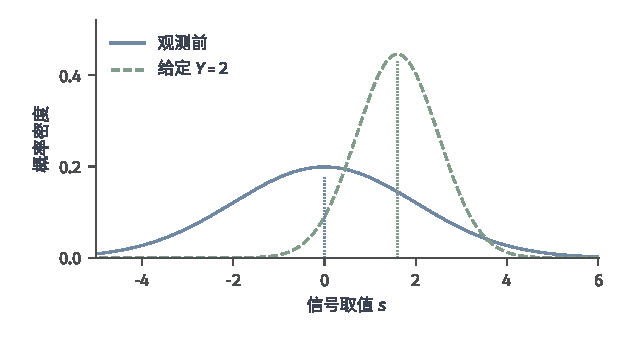
\includegraphics[width=105mm]{figures/02-mathematical-preliminaries-lower/01-random-variables-distributions-and-causality/matplotlib/probability-gaussian-observation-update/figure.pdf}
  \caption{独立高斯噪声下的一次观测更新。信号\(S\sim\mathcal N(0,4)\)，观测\(Y=S+\varepsilon\)，其中\(\varepsilon\sim\mathcal N(0,1)\)与\(S\)独立。蓝实线为\(S\)的先验密度，绿虚线为给定\(Y=2\)后的\(\mathcal N(1.6,0.8)\)密度；细竖线标出两者均值。}
  \label{fig:probability-gaussian-observation-update}
\end{figure}

多元高斯分布是一个特殊情形：联合高斯随机向量的两个子向量若协方差为零，则它们独立；条件高斯中的条件协方差为零也对应条件独立。这个结论依赖高斯
分布由一、二阶矩完全确定，不能推广到一般分布。


\subsubsection{高斯密度的乘积与多源信息合并}
\label{sec:probability-gaussian-density-products}
单个观测通过条件化改变高斯分布。若多项信息都以同一个未知量上的高斯密度表达，把这些密度相乘并归一化，也能得到闭式结果。这里相乘的是同一取值\(\bm x\)上的函数，并不是把多个随机向量相加。

\begin{theorem}[高斯密度乘积]
\label{prop:probability-gaussian-density-product}
设\(m\geq1\)，\(p_j\)是\(\mathbb R^d\)上均值\(\bm\mu_j\)、正定协方差\(\bm\Sigma_j\)的高斯密度。记精度矩阵\(\bm\Lambda_j=\bm\Sigma_j^{-1}\)。则
\[
 q(\bm x)=\frac{\prod_{j=1}^m p_j(\bm x)}{\int_{\mathbb R^d}\prod_{j=1}^m p_j(\bm z)\,\mathrm d\bm z}
\]
是高斯密度，其协方差与均值分别为
\begin{equation}
 \bm\Sigma=\left(\sum_{j=1}^m\bm\Lambda_j\right)^{-1},
 \qquad
 \bm\mu=\bm\Sigma\sum_{j=1}^m\bm\Lambda_j\bm\mu_j.
 \label{eq:probability-gaussian-density-product}
\end{equation}
\end{theorem}

\begin{proof}
乘积中各高斯指数的二次型之和为
\[
 \sum_j(\bm x-\bm\mu_j)^\top\bm\Lambda_j(\bm x-\bm\mu_j)
 =\bm x^\top\bm\Lambda\bm x-2\bm x^\top\bm h+c,
\]
其中\(\bm\Lambda=\sum_j\bm\Lambda_j\)、\(\bm h=\sum_j\bm\Lambda_j\bm\mu_j\)，\(c\)与\(\bm x\)无关。正定矩阵之和仍正定，因此可以配方为
\[
 (\bm x-\bm\Lambda^{-1}\bm h)^\top\bm\Lambda
 (\bm x-\bm\Lambda^{-1}\bm h)+c-\bm h^\top\bm\Lambda^{-1}\bm h.
\]
以该二次型构成的高斯函数关于\(\bm x\)的积分为有限正数。归一化以后，常数项相消，余下的密度正是式~\eqref{eq:probability-gaussian-density-product}中的高斯密度。
\end{proof}

一维时，均值按\(1/\sigma_j^2\)加权，方差为\((\sum_j1/\sigma_j^2)^{-1}\)。例如两个方差均为\(1\)、均值分别为\(0\)和\(2\)的密度，归一化乘积为\(\mathcal N(1,1/2)\)。乘积给出的方差变小，并不自动证明两项信息一致：即使把第二个均值改成\(10\)，方差仍为\(1/2\)。若数据来源存在相关性、模型失配或相互冲突，单凭这个代数运算不能把缩小的方差解释为可靠的推断精度。

多源后验合并还要检查先验是否重复计算。设\(\Theta\)有先验密度\(p_0\)，观测\(Y_1,\ldots,Y_m\)给定\(\Theta\)后条件独立，且各单源后验\(p_j(\theta\mid y_j)\)都采用同一个先验。由Bayes公式，在\(p_0(\theta)>0\)的支持上，
\begin{equation}
 p(\theta\mid y_1,\ldots,y_m)
 \propto p_0(\theta)\prod_jp(y_j\mid\theta)
 \propto p_0(\theta)^{1-m}\prod_jp_j(\theta\mid y_j).
 \label{eq:probability-common-prior-posterior-fusion}
\end{equation}
每个单源后验都含有一次先验；直接把它们相乘会把先验计入\(m\)次，因此要除去多出的\(m-1\)次。这个推导要求给定未知量后的条件独立，并要求所用后验、似然和归一化积分有定义。任意给出的高斯密度乘积总能按上面的命题归一化，但未必代表某组真实观测的共同后验。

\subsection{基于指数族的参数化表示}
% Baseline P:1018-1081
Poisson计数和高斯读数具有不同的取值空间，但其密度中的参数依赖都能集中到少量摘要与一个归一化项。指数族把这种共同结构写出来，使均值、协方差和似然计算能够复用同一组公式。
\begin{definition}[指数族]
  \label{def:probability-exponential-family}
在可测空间上固定一个\(\sigma\)有限参考测度\(\mu\)，非负可测基准项\(h\)和可测向量函数\(\bm T\)。一类由\(\bm{\eta}\)索引的分布若都被
\(\mu\)支配，且能写成
\begin{equation}
  \frac{\mathrm{d}P_{\bm{\eta}}}{\mathrm{d}\mu}(x)
  =
  h(x)\exp\left\{
    \bm{\eta}^{\top}\bm{T}(x)-A(\bm{\eta})
  \right\},
  \label{eq:probability-exponential-family}
\end{equation}
就称为\term{指数族}（exponential family）。其中\(\bm{\eta}\)是\term{自然参数}，\(\bm{T}(x)\)是充分统计量，\(h(x)\)是基准项。负责归一化的对数配分函数为
\[ A(\bm{\eta})
  =\log\int h(x)e^{\bm{\eta}^{\top}\bm{T}(x)}\,\mathrm{d}\mu(x), \]
自然参数空间由该积分严格为正且有限的参数组成；所用参数集合可以是这个空间的子集。
\end{definition}
这里“充分”可以先理解为：
样本取值中与参数\(\bm{\eta}\)有关的部分只通过摘要\(\bm{T}(x)\)进入密度；对独立同分布样本，相应摘要是
\(\sum_i\bm{T}(x_i)\)。充分性的正式定义与判据留到第~\ref{sec:statistics-likelihood-robustness}节。

离散分布通常取计数测度，此时积分就是求和；具有Lebesgue密度的分布取Lebesgue测度。因而Poisson分布与高斯分布都能由同一形式描述，但使用的参考测度不同。

若\(\bm{\eta}\)位于自然参数空间内部，并存在可积控制函数允许交换微分与积分，则
\[
\begin{aligned}
  \nabla A(\bm{\eta})
  &=
  \frac{\int \bm{T}(x)h(x)
  e^{\bm{\eta}^{\top}\bm{T}(x)}\,\mathrm{d}\mu(x)}
  {\int h(x)e^{\bm{\eta}^{\top}\bm{T}(x)}\,\mathrm{d}\mu(x)}\\
  &=
  \mathbb{E}_{\bm{\eta}}[\bm{T}(X)].
\end{aligned}
\]
再求一次导数得到
\begin{equation}
  \nabla^2 A(\bm{\eta})
  =
  \operatorname{Cov}_{\bm{\eta}}(\bm{T}(X)).
  \label{eq:probability-log-partition-hessian}
\end{equation}
自然参数空间的凸性来自Hölder不等式：两个有限归一化积分的几何插值仍有限。上述Hessian半正定进一步说明\(A\)在参数空间内部的凸性。若存在非零\(\bm a\)，使
\(\bm a^\top\bm T(X)\)几乎处处为常量，该方向的方差为零，Hessian矩阵就奇异。
这包括某个统计量恒为常量，以及一个统计量等于其余统计量的线性组合再加常数的情况；
严格凸性并不自动成立。

以Poisson分布为例，把密度写成\eqref{eq:probability-exponential-family}的形式即可读出参数：
\[ p_\lambda(x)
  =\frac{1}{x!}\exp\{x\log\lambda-\lambda\}. \]
自然参数为\(\eta=\log\lambda\)，充分统计量为\(T(x)=x\)，
基准项为\(h(x)=1/x!\)，配分函数为\(A(\eta)=e^\eta\)。于是
\[ A'(\eta)=e^\eta=\mathbb{E}X,
  \qquad A''(\eta)=e^\eta=\operatorname{Var}(X), \]
与Poisson分布的均值、方差一致。

这一步的做法可以固定下来：先整理指数部分，让参数只以「参数乘统计量」的乘积形式出现，
剩下的\(x\)部分归入\(h(x)\)，剩余常量归入\(A(\bm\eta)\)。按这个顺序核对下面两例，
就能看出\(A\)的导数为什么恰好给出矩。

Bernoulli分布提供另一个核对。取\(0<p<1\)，令\(\eta=\log(p/(1-p))\)，则
\[
  p_\eta(x)=\exp\{x\eta-\log(1+e^\eta)\},
  \qquad x\in\{0,1\}.
\]
所以\(A(\eta)=\log(1+e^\eta)\)，
\(A'(\eta)=p\)、\(A''(\eta)=p(1-p)\)，仍与Bernoulli分布的矩一致。
这里\(h(x)=1\)，全部参数依赖都进了指数，因此\(A\)必须同时承担归一化与矩计算两项任务。

已知方差\(\sigma^2>0\)的高斯分布更能说明\(h\)的作用。把密度指数上的平方展开为
\[
  -\frac{(x-\mu)^2}{2\sigma^2}
  =\frac{\mu}{\sigma^2}x-\frac{x^2}{2\sigma^2}-\frac{\mu^2}{2\sigma^2},
\]
第一项已经是「参数乘\(x\)」的形式，取\(\eta=\mu/\sigma^2\)、\(T(x)=x\)；第二项只含\(x\)，
归入基准项\(h(x)=\exp\{-x^2/(2\sigma^2)\}/\sqrt{2\pi\sigma^2}\)；第三项只含参数，移入配分函数得到
\(A(\eta)=\sigma^2\eta^2/2\)。于是
\(A'(\eta)=\sigma^2\eta=\mu\)、\(A''(\eta)=\sigma^2\)，均值与方差都被读出。
同一个分布的另一种抽样方式——多次独立观察——只需把\(T(x)\)换成样本和，
指数部分因此可加；这正是后文在独立样本下直接对统计量求和的原因。

这些例子说明，产生均值和协方差的是
\(\log\)配分函数\(A\)的导数，不是未取对数的归一化常数本身。写代码或查表时容易把两者
混用：密度前面的系数常随参数变化，但由它出发求导得不到矩，必须先把参数依赖整理进指数。

\section{随机变量的变换与生成}
\label{sec:rv-transformations}
\label{sec:probability-random-vectors-transformations}
由读数得到新随机对象，可以改变映射，也可以改变生成规律。把两台设备的读数相加，固定的是共同概率空间，变化的是取值函数；先确定设备状态再生成噪声，需要额外给出条件抽样规则；保持读数映射不变而重新分配事件概率，则改变基础权重。三种操作分别改变取值映射、条件生成规则与概率权重；随机序列和过程由第~\ref{chap:random-sequences-and-processes}章另行展开。

\subsection{基于取值映射的变换}
把几个读数合成一个新读数，是实际计算中最常见的操作：把两台设备的读数相加、相减，
取两者的最大或最小，都需要知道结果的分布。下面的规则先处理任意可测变换，
再给出可以逐项验算的情形。

\subsubsection{分布变换的一般规则}
\label{sec:rv-pushforward}
若\(X\)取值于\((E,\mathcal E)\)，\(g:E\to F\)可测，则
\(Y=g(X)\)的分布是\(P_Y=g_\#P_X\)，即
\[
P_Y(B)=P_X(g^{-1}(B)),\qquad
\mathbb E h(Y)=\int_E h(g(x))\,P_X(\mathrm dx)
\]
对非负可测\(h\)或可积\(h\)成立。这个规则不要求密度，也不要求\(g\)可逆。
% Baseline P:1187-1202
以下限制为同维欧氏空间：设\(\mathcal X,\mathcal Y\subseteq\mathbb R^d\)为开集，
\(\bm X\)在\(\mathcal X\)上相对于\(d\)维Lebesgue测度具有密度\(f_{\bm X}\)，
\(g:\mathcal X\to\mathcal Y\)为\(C^1\)微分同胚，即双射且它与逆映射都连续可微。
令\(\bm Y=g(\bm X)\)，换元公式给出输出相对于同维Lebesgue测度的密度
\begin{equation}
  f_{\bm{Y}}(\bm{y})
  =
  f_{\bm{X}}\bigl(g^{-1}(\bm{y})\bigr)
  \left|
    \det\bm{J}_{g^{-1}}(\bm{y})
  \right|.
  \label{eq:probability-density-change-variables}
\end{equation}
Jacobian矩阵的行列式补偿局部体积变化。只把\(x=g^{-1}(y)\)代入原密度而漏掉该因子，所得函数通常不能积分为\(1\)。

若映射可分为有限或可数个一一对应的\(C^1\)分支，各分支Jacobian非零，则在正则值处把各逆像分支的换元密度相加。一般可测映射仍应从推送测度定义出发。例如\(Y=X^2\)且\(X\)有密度时，对\(y>0\)，
\[ f_Y(y)
  =\frac{f_X(\sqrt{y})+f_X(-\sqrt{y})}{2\sqrt{y}}. \]
输出密度必须相对于输出空间的参考测度定义。输入与输出维数不同时，非方阵Jacobian不能直接取行列式换元。若
\((X_1,X_2)\)在单位正方形上均匀分布，投影\(g(x_1,x_2)=x_1\)降到一维，输出仍有一维密度\(1_{[0,1]}\)，由对\(x_2\)积分得到。相反，嵌入\(h(x)=(x,x)\)把一维变量放入二维，像落在直线上，没有二维Lebesgue密度。应比较输出支持与输出空间的维数，而不能把“降维”直接等同于“没有密度”。

\paragraph{概率积分变换与分位数复合}
\label{sec:probability-integral-transform}
换元公式逐点计算输出密度。有时只希望把一个已知分布改成另一个分布，可以先把输入变成累积概率，再用目标分位数把概率映回读数。这条路径直接使用分布函数，不需要对密度求导。

\begin{theorem}[概率积分变换与逆分位数生成]
\label{prop:probability-integral-transform}
若实随机变量\(X\)的分布函数\(F\)连续，则\(F(X)\sim\operatorname{Unif}[0,1]\)。对任意实数轴分布函数\(G\)，令\(G^{-1}(u)=\inf\{y:G(y)\geq u\}\)，其中\(0<u<1\)。若\(U\sim\operatorname{Unif}[0,1]\)，则\(G^{-1}(U)\)具有分布函数\(G\)。因此，当\(F\)连续时，\(G^{-1}(F(X))\)具有目标分布\(G\)；零概率的端点事件上可任取约定值。
\end{theorem}

\begin{proof}
固定\(0<u<1\)。由连续性及两端极限，集合\(\{x:F(x)\leq u\}\)有有限上端点\(b_u\)，并有\(F(b_u)=u\)。单调性给出\(\{F(X)\leq u\}=\{X\leq b_u\}\)，故其概率等于\(u\)。这证明第一条结论；证明不要求\(F\)严格递增，平坦区间不承载额外概率。

对目标分位数，分布函数的右连续性保证\(G^{-1}(u)\leq y\)当且仅当\(u\leq G(y)\)。所以
\[
 \mathbb P(G^{-1}(U)\leq y)=\mathbb P(U\leq G(y))=G(y),
\]
得到第二条结论。将第一条产生的均匀变量代入，便得到分位数复合结论。
\end{proof}

例如\(X\sim\operatorname{Unif}[0,2]\)时，\(F(X)=X/2\)。取目标为速率\(\lambda>0\)的指数分布，其分位数为\(G^{-1}(u)=-\log(1-u)/\lambda\)，于是\(-\log(1-X/2)/\lambda\)服从该指数分布。前一变换统一概率尺度，后一变换指定输出尺度。

若\(F\)有跳跃，\(F(X)\)一般不均匀。例如等概率取零或一的\(X\)，经过\(F\)后只取\(1/2\)与\(1\)，不会产生连续均匀分布。图像直方图均衡与匹配可借用这一构造，但有限灰度级的确定性映射不能把每个原子任意拆分，通常只能近似实现均衡；不能把连续情形的精确结论原样套用到离散直方图。

\subsubsection{随机变量的组合与排序}
\label{sec:rv-combinations}
把两个读数相加或加权组合，结果的不确定程度是多少？平均值可以直接相加，波动却要
看两部分的共同变化。
可积变量的和满足\(\mathbb E(X+Y)=\mathbb EX+\mathbb EY\)，不需要独立；
二阶可积时
\[
\operatorname{Var}(aX+bY)
=a^2\operatorname{Var}(X)+b^2\operatorname{Var}(Y)
 +2ab\operatorname{Cov}(X,Y).
\]
第三项就是共同变化带来的修正：同向变化时相加，反向变化时相消。
图~\ref{fig:rv-dependence}中三个和的方差依次为\(1,1/2,0\)。相同边缘并没有给出相同的累计波动。若只知两个变量可积，乘积未必可积；二阶可积则由Cauchy--Schwarz保证乘积可积。比值还须确保分母非零，且另查比值的矩。

\paragraph{信号相关噪声的均值与方差}
固定非负信号强度\(x\)，设读数为
\[
 Y=\alpha N+\varepsilon,\qquad
 N\sim\operatorname{Poisson}(x/\alpha),\qquad
 \varepsilon\sim\mathcal N(0,\sigma^2),
\]
其中\(\alpha>0\)、\(\sigma^2>0\)，且\(N\)与\(\varepsilon\)独立。\(N\)表示随机计数，\(\alpha\)把一次计数换算为读数增量，\(\varepsilon\)表示独立的加性读出误差；当\(x=0\)时约定\(N=0\)几乎处处。这个泊松—高斯噪声（Poisson–Gaussian noise）模型可用于近似描述尚未经过复杂处理的传感器读数\scite{vision-foi2008}。

Poisson变量的均值与方差均为\(x/\alpha\)，独立性又使交叉协方差为零，因而
\begin{equation}
 \mathbb E Y=x,\qquad
 \operatorname{Var}(Y)=\alpha x+\sigma^2,
 \qquad
 \mathbb E[(Y-x)^2]=\alpha x+\sigma^2.
 \label{eq:probability-poisson-gaussian-moments}
\end{equation}
最后一项是读数相对固定信号\(x\)的均方误差；这里均值等于目标，所以它与方差相等。即使加性读出噪声方差固定，总误差方差仍随信号增加。作为教学计算，取\(\alpha=1\)、\(\sigma=2\)，\(x=4\)与\(x=100\)的标准差分别为\(\sqrt8\)与\(\sqrt{104}\)，信号除以标准差分别约为\(1.41\)与\(9.81\)。绝对波动增大与相对误差降低可以同时发生；不能用一个固定方差的加性噪声模型覆盖这两个强度下的规律。


\paragraph{相关读数的加权组合}
这一修正对重复测量的效果值得单独算一次。设两次读数\(X_1,X_2\)同方差
\(\operatorname{Var}(X_i)=\sigma^2\)、相关系数为\(\rho\)，取两者平均
\(\bar X=(X_1+X_2)/2\)。按上式取\(a=b=1/2\)，得
\[
  \operatorname{Var}(\bar X)
  =\frac{\sigma^2}{4}+\frac{\sigma^2}{4}
   +2\cdot\frac14\rho\sigma^2
  =\frac{\sigma^2(1+\rho)}2.
\]
\(\rho=0\)时方差降为一半，这正是“多测几次更准”的依据；\(\rho=1\)时结果是
\(\sigma^2\)，与只测一次无异。只报告样本量而不报告相关性，就无法判断平均是否
真的降低了波动，这也说明成批出现的测量偏差无法靠增多样本消除。权重不等时第二项按
权重平方减少、第三项按权重乘积变化，两者比例不同，因此可靠但相关的读数应当给予
多少权重，需要代入具体数值比较，不能只凭哪一次读数更可靠来判断。

\paragraph{和、乘积与比值的分布}
若\(X,Y\)具有联合密度\(f_{X,Y}\)，换元与边缘化给出
\[
\begin{aligned}
f_{X+Y}(s)&=\int_{\mathbb R}f_{X,Y}(x,s-x)\,\mathrm dx,\\
f_{XY}(z)&=\int_{\mathbb R\setminus\{0\}}
 f_{X,Y}(x,z/x)\frac{\mathrm dx}{|x|},\\
f_{X/Y}(r)&=\int_{\mathbb R}|y|f_{X,Y}(ry,y)\,\mathrm dy.
\end{aligned}
\]
后两式的Jacobian因子分别为\(1/|x|\)和\(|y|\)。独立时联合密度可分解，和的密度便是卷积\(f_X*f_Y\)；离散和相应使用
\(\mathbb P(X+Y=s)=\sum_x\mathbb P(X=x)\mathbb P(Y=s-x)\)。
例如独立标准高斯之比\(R=X/Y\)满足
\[
f_R(r)=\frac1{2\pi}\int_{\mathbb R}|y|
 e^{-(1+r^2)y^2/2}\,\mathrm dy
=\frac1{\pi(1+r^2)}.
\]
这是标准Cauchy密度，\(\mathbb E|R|=\infty\)。分子分母都拥有全部矩，也不保证比值有均值。

\paragraph{独立和的变换函数}
独立性还把变换函数化为乘积：
\[
\varphi_{X+Y}(t)=\mathbb E(e^{\mathrm itX}e^{\mathrm itY})
=\varphi_X(t)\varphi_Y(t).
\]
在矩母函数共同有限的邻域，同样有
\(M_{X+Y}=M_XM_Y\)、\(K_{X+Y}=K_X+K_Y\)。向量的独立坐标使联合累积量生成函数按坐标相加，因此所有涉及至少两个不同坐标的累积量都为零。
反过来，若联合累积量生成函数在原点邻域解析，且这些跨坐标累积量全部为零，其Taylor展开就没有混合项。
又因\(K_{\bm X}(\bm0)=0\)，剩下的各组单坐标项分别等于边缘累积量生成函数，从而
\[
 K_{\bm X}(\bm t)=\sum_jK_{X_j}(t_j),\qquad
 M_{\bm X}(\bm t)=\prod_jM_{X_j}(t_j).
\]
右侧也是边缘乘积测度的矩母函数；由定理~\ref{thm:rv-transform-uniqueness}，联合分布等于该乘积测度，故坐标独立。
这里只让有限几个混合累积量为零还不够。高阶累积量可识别协方差未反映的非高斯依赖，纯高斯的三阶及以上累积量则为零。
独立Poisson变量的矩母函数为
\(\exp\{\lambda(e^t-1)\}\)，相乘后参数相加；独立标准高斯平方的Gamma矩母函数相乘，则得到前面定义的卡方分布。

\paragraph{仿射变换与白化}
对向量，令\(\bm Y=\bm A\bm X+\bm b\)，相应矩存在时
\[
\mathbb E\bm Y=\bm A\bm\mu+\bm b,\quad
\operatorname{Cov}(\bm Y)=\bm A\bm\Sigma\bm A^\top,\quad
\operatorname{Cov}(\bm A\bm X,\bm B\bm X)=\bm A\bm\Sigma\bm B^\top.
\]
前两条不要求高斯性。若\(\bm X\)联合高斯，则任意线性组合仍高斯，因而
\(\bm Y\sim\mathcal N(\bm A\bm\mu+\bm b,\bm A\bm\Sigma\bm A^\top)\)，即使\(\bm A\)不满秩也成立，但不能因此写出非退化密度。

协方差变换式也说明了白化（whitening）的含义：对中心化向量作线性变换，使协方差成为单位阵。若\(\bm\Sigma\succ\bm0\)，可取
\(\bm Y=\bm\Sigma^{-1/2}(\bm X-\bm\mu)\)；此后任何正交旋转\(\bm Q\bm Y\)仍有单位协方差，因为\(\bm Q\bm I\bm Q^\top=\bm I\)。
因此二阶统计量无法继续辨认这些旋转方向。独立成分分析（independent component analysis, ICA）希望从若干源信号的线性混合观测中，辨认相互独立的源。
源具有适当的非高斯性时，高阶统计量可以提供白化后仍缺少的方向信息；纯高斯的三阶及以上累积量全为零，不能承担这一任务。这里说明的是高阶信息的用途，并不保证任意三阶、四阶量都足以唯一识别源。

\paragraph{排序与顺序统计量}
排序也是函数变换。取正整数\(n\)和\(1\leq k\leq n\)。若\(X_1,\ldots,X_n\)独立同分布，分布函数为\(F\)，则
\[
\mathbb P(\max_iX_i\leq x)=F(x)^n,\quad
\mathbb P(\min_iX_i>x)=(1-F(x))^n,
\]
\[
\mathbb P(X_{(k)}\leq x)
=\sum_{j=k}^n\binom njF(x)^j(1-F(x))^{n-j}.
\]
这里把“第\(k\)小不超过\(x\)”改写成至少\(k\)个输入不超过\(x\)，所以出现二项计数。
% Baseline T:963-968
对次序统计量\(Y_{(1)}\leq\cdots\leq Y_{(n)}\)，经验分位数由相应秩位置给出。
若\(Y_1,\ldots,Y_n\)是来自连续分布\(F\)的独立同分布样本，则
\(F(Y_{(k)})\)服从
\(\operatorname{Beta}(k,n+1-k)\)，因此可以用秩而不是高斯近似构造分位数区间。
对离散或混合分布，跳跃与平坦区间都要求覆盖计算保留定义中的不等式方向。

\subsection{基于条件分布的随机生成}
\label{sec:rv-random-generation}
\subsubsection{基于类别选择的混合生成}
% Baseline P:1206-1253
有时读数来自几类未直接标记的来源，例如同一批产品由两条产线分别生产，误差规律并不相同。混合模型先抽取离散指标\(Z\)表示来自哪一类，再从该类的分量分布生成\(X\)：
\[ p(x)=\sum_{k=1}^{K}\mathbb{P}(Z=k)p(x\mid Z=k). \]
边缘化\(Z\)得到混合密度，条件化\(X\)则得到分量责任概率。潜变量不必对应可观测的真实类别；它本质上是组织联合分布和计算的数学变量。

混合分布的方差同时包含分量内和分量间变化。若
\(\mathbb{P}(Z=1)=1/4\)、\(\mathbb{P}(Z=2)=3/4\)，且
\[
  X\mid Z=1\sim\mathcal{N}(-1,1),\qquad
  X\mid Z=2\sim\mathcal{N}(1,1),
\]
则\(\mathbb{E}X=(-1)/4+3/4=1/2\)。全方差公式给出
\[
  \operatorname{Var}(X)
  =\underbrace{\mathbb{E}[\operatorname{Var}(X\mid Z)]}_{1}
   +\underbrace{\operatorname{Var}(\mathbb{E}[X\mid Z])}_{3/4}
  =\frac74.
\]
只平均两个分量方差会漏掉均值差造成的\(3/4\)。

\subsubsection{基于随机参数的层次生成}
有限混合用类别指标选择分量。若要让多个读数共享一个随机参数，可以先生成该参数，再按参数所决定的条件分布生成有限个读数。这样的层次模型（hierarchical model）把参数本身也作为随机对象，例如
\[ \Theta\sim\pi,\qquad
  X_i\mid\Theta\mathrel{\overset{\mathrm{ind}}{\sim}}p_\Theta,\qquad i=1,\ldots,n. \]
给定\(\Theta\)时，观测条件独立；边缘化共同参数后，观测通常相关。把“条件独立”
误写成“边缘独立”会丢掉层次模型中共享不确定性的主要作用。有限混合也能写成一类层次构造；这里的区别是当前把哪一项作为条件，以及多个读数是否共享这项条件。

例如设\(\Theta\)具有有限正方差，令\(X_1=\Theta+\varepsilon_1\)、\(X_2=\Theta+\varepsilon_2\)，其中两个噪声零均值、二阶可积，且彼此独立并独立于\(\Theta\)。给定\(\Theta\)后，两项噪声仍独立，所以\(X_1,X_2\)条件独立；不固定该参数时，展开协方差得到\(\operatorname{Cov}(X_1,X_2)=\operatorname{Var}(\Theta)>0\)。条件内的生成规则与条件之间的共同变化因此承担不同作用。

\subsection{基于概率重加权的分布变换}

保持同一个取值函数\(g\)，把事件权重从\(\mu\)改成\(\nu\)，会改变它的积分。若\(\nu\ll\mu\)，第~\ref{sec:probability-radon-nikodym-change-measure}节已经给出密度比\(r\)。现在把这个比值直接乘入旧积分，便能计算新权重下的平均。
\label{sec:rv-change-measure}
\subsubsection{密度比与换测度积分}
% Baseline P:249-302
\begin{theorem}[换测度积分公式]
\label{thm:probability-change-measure-integral}
若\(\nu\ll\mu\)，\(r=\mathrm{d}\nu/\mathrm{d}\mu\)，则对每个非负可测函数\(g\)，
\[ \int g\,\mathrm{d}\nu
  =\int gr\,\mathrm{d}\mu. \]
只要\(g\)在\(\nu\)下可积，同一等式也对实值\(g\)成立。
\end{theorem}

\begin{proof}
对指示函数\(g=\mathbb{I}_A\)，结论就是Radon--Nikodym表示。由线性性，它对非负简单函数成立。任取非负可测\(g\)，选择简单函数\(g_n\uparrow g\)，分别在
\(\nu\)和\(\mu\)下使用单调收敛定理即可。对可积实值函数，再分别处理\(g^+\)与\(g^-\)。
\end{proof}

密度比存在、有界和具有有限二阶矩是三项不同条件。若\(P\ll Q\)，则\(w=\mathrm{d}P/\mathrm{d}Q\)存在且\(\mathbb{E}_Q[w]=1\)，但这不推出
\(\lVert w\rVert_\infty<\infty\)，也不推出\(\mathbb{E}_Q[w^2]<\infty\)。例如在\((0,1)\)上令\(Q\)为均匀分布，取
\[ w(x)=\frac{1}{2\sqrt{x}}. \]
它的积分为\(1\)，所以定义一个\(P\ll Q\)；但\(w\)无界，且\(\int_0^1w(x)^2\,\mathrm{d}x=\infty\)。换测度恒等式仍成立，使用该权重的蒙特卡洛估计却可能没有有限方差。

有限表可以直接核对权重方向。设参考分布\(Q\)在三个结果上的概率为
\((0.5,0.4,0.1)\)，目标分布\(P\)为\((0.2,0.3,0.5)\)，则
\[
  w=\frac{\mathrm{d}P}{\mathrm{d}Q}=(0.4,0.75,5).
\]
对取值\(g=(1,2,4)\)，有
\[
  \mathbb{E}_P[g]=2.8
  =0.5(0.4)(1)+0.4(0.75)(2)+0.1(5)(4)
  =\mathbb{E}_Q[wg].
\]
第三个结果在\(Q\)下少见，却在\(P\)下承载一半质量，所以产生大权重。若把参考概率
\(0.1\)改成\(0\)而保持目标概率\(0.5\)，则\(P\not\ll Q\)，任何重加权都无法从
\(Q\)样本恢复这部分目标质量。

图~\ref{fig:probability-importance-weights}显示，权重改变的是每个结果对平均的贡献，而不是把观测值\(g_j\)解释为概率。未加权平均为\(1.7\)，加权平均为\(2.8\)；第三个结果的贡献从\(0.4\)增至\(2\)，也预示它偶尔出现时会显著推动估计值。

\begin{figure*}[htbp]
  \centering
  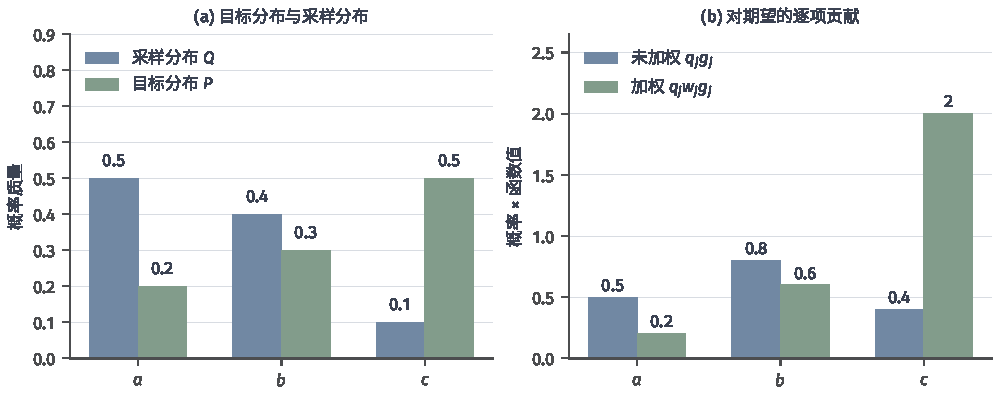
\includegraphics[width=\linewidth]{figures/02-mathematical-preliminaries-lower/01-random-variables-distributions-and-causality/matplotlib/probability-importance-weights/figure.pdf}
  \caption{三结果换测度的有限构造。左图比较采样分布\(Q\)与目标分布\(P\)，右图比较\(q_jg_j\)与\(q_jw_jg_j=p_jg_j\)。各柱从零起画；右图柱高之和分别为\(1.7\)和\(2.8\)，并非单点概率。}
  \label{fig:probability-importance-weights}
\end{figure*}

绝对连续性也决定几乎处处结论能否转移。若\(P\ll Q\)，且
\(|g|\leq M\)在\(Q\)下几乎处处成立，则违背上界的集合是\(Q\)-零集，因而也是
\(P\)-零集；同一上界在\(P\)下仍成立。反向转移需要\(Q\ll P\)，不能只凭
\(P\ll Q\)得到。若\(|g|\leq B\)，则
\[
  \mathbb{E}_Q[w^2g^2]\leq B^2\mathbb{E}_Q[w^2],
\]
所以权重二阶矩有限是有界被积函数获得有限重加权方差的充分条件。把权重截为
\(w_c=\min\{w,c\}\)会限制波动，但
\(\mathbb{E}_Q[w_cg]\)与\(\mathbb{E}_P[g]\)之差为
\(-\mathbb{E}_Q[(w-c)_+g]\)，一般不为零。

\subsubsection{条件期望的重加权与归一化}
% Baseline P:628-716
设\(Q\ll P\)，并记\(L=\mathrm{d}Q/\mathrm{d}P\)。对\(X\in L^1(Q)\)，在\(\mathbb{E}_P[L\mid\mathcal{G}]>0\)处有
\begin{equation}
  \mathbb{E}_Q[X\mid\mathcal{G}]
  =
  \frac{\mathbb{E}_P[LX\mid\mathcal{G}]}
       {\mathbb{E}_P[L\mid\mathcal{G}]}.
  \label{eq:probability-conditional-change-measure}
\end{equation}
为验证这个候选变量确实是条件期望，记
\[
  D=\mathbb{E}_P[L\mid\mathcal{G}],
  \qquad
  N=\mathbb{E}_P[LX\mid\mathcal{G}],
\]
并在\(\{D>0\}\)上令\(Z=N/D\)，在\(\{D=0\}\)上令\(Z=0\)。分母零集在\(Q\)下可以忽略，因为
\[
  Q(D=0)
  =
  \mathbb{E}_P[L\mathbb{I}\{D=0\}]
  =
  \mathbb{E}_P[D\mathbb{I}\{D=0\}]
  =0.
\]
条件期望的单调性还给出
\[
  |N|
  \leq
  \mathbb{E}_P[L|X|\mid\mathcal{G}].
\]
在\(\{D=0\}\)上，非负变量\(L\mathbb{I}\{D=0\}\)的期望为零，因而\(L=0\)几乎处处。于是
\[
  \mathbb{E}_P\left[
    \mathbb{E}_P[L|X|\mid\mathcal{G}]
    \mathbb{I}\{D=0\}
  \right]
  =
  \mathbb{E}_P[L|X|\mathbb{I}\{D=0\}]
  =0,
\]
上面的条件三角不等式进而说明\(N=0\)在\(\{D=0\}\)上几乎处处成立。因此\(DZ=N\)几乎处处，而且
\[
  \begin{aligned}
    \mathbb{E}_Q|Z|
    &=
    \mathbb{E}_P[L|Z|]
    =
    \mathbb{E}_P[D|Z|]\\
    &=
    \mathbb{E}_P\bigl[|N|\mathbb{I}\{D>0\}\bigr]
    \leq
    \mathbb{E}_P[L|X|]
    =
    \mathbb{E}_Q|X|<\infty.
  \end{aligned}
\]
这里把\(\mathcal{G}\)-可测的非负因子\(|Z|\)提出条件期望，可以由有界截断和单调收敛得到。候选变量的可积性建立后，对
\(A\in\mathcal{G}\)可合法地计算
\[
  \begin{aligned}
    \int_A Z\,\mathrm{d}Q
    &=
    \int_A ZL\,\mathrm{d}P
    =
    \int_A Z\mathbb{E}_P[L\mid\mathcal{G}]\,\mathrm{d}P\\
    &=
    \int_A \mathbb{E}_P[LX\mid\mathcal{G}]\,\mathrm{d}P
    =
    \int_A LX\,\mathrm{d}P
    =
    \int_A X\,\mathrm{d}Q.
  \end{aligned}
\]
因此\(Z\)满足\(X\)在\(Q\)下关于\(\mathcal{G}\)的条件期望定义。公式\eqref{eq:probability-conditional-change-measure}是Bayes更新的一般测度形式；
分母零集与候选变量可积性都需要像上面这样核对。

用有限分组可以看出分母为何不可省略。设参考分布\(P\)把四个结果
\(\omega_1,\ldots,\omega_4\)分别赋予概率\((0.4,0.1,0.1,0.4)\)，目标分布
\(Q\)赋予\((0.1,0.5,0.1,0.3)\)。令信息\(\mathcal{G}\)只区分
\(A=\{\omega_1,\omega_2\}\)和\(A^{\mathsf c}\)，并令
\(X=(0,1,0,1)\)。权重\(L\)在四点上的值为\((0.25,5,1,0.75)\)。在\(A\)内，
\[
  \mathbb{E}_P[LX\mid\mathcal{G}]
  =\frac{0.5}{0.5}=1,\qquad
  \mathbb{E}_P[L\mid\mathcal{G}]
  =\frac{0.1+0.5}{0.5}=1.2,
\]
所以目标条件均值为\(1/1.2=5/6\)，与
\(\mathbb{E}_Q[X\mid A]=0.5/(0.1+0.5)\)一致。
省略分母却会得到\(1\)，可以直接看到重新归一化改变了答案。
在\(A^{\mathsf c}\)内，分子为\(0.3/0.5=0.6\)，分母为\(0.4/0.5=0.8\)，
相除得到\(3/4\)，也等于该组在\(Q\)下的条件均值。
条件化后必须按每个信息分组的目标总质量分别归一化。

\section{单个随机变量的尾概率控制}
\label{sec:probability-elementary-tail-bounds}
\subsection{非负随机变量的Markov不等式}
如果一个非负随机变量经常超过阈值，它的平均值就不能太小。这一关系使我们能从已知的一阶矩控制大取值事件。设非负随机变量为\(X\)，阈值为\(a>0\)，则
\begin{equation}
  \mathbb{P}(X\geq a)
  \leq
  \frac{\mathbb{E}X}{a}.
  \label{eq:probability-markov-inequality}
\end{equation}
证明只需写
\(\mathbb{E}X\geq
\mathbb{E}[X\mathbb{I}\{X\geq a\}]
\geq a\mathbb{P}(X\geq a)\)。
这就是Markov不等式。

\subsection{有限方差下的Chebyshev不等式}
对均值\(\mu\)、方差\(\sigma^2<\infty\)的随机变量，把
Markov不等式用于\((X-\mu)^2\)，得到Chebyshev不等式
\begin{equation}
  \mathbb{P}(|X-\mu|\geq t)
  \leq\frac{\sigma^2}{t^2},
  \qquad t>0.
  \label{eq:probability-chebyshev-inequality}
\end{equation}
它只使用二阶矩，因而适用范围广，但没有利用有界性或指数矩信息。

\section{本章小结}
\label{sec:probability-summary}
传感器的一次读数既是一项确定的取值规则，也是在概率空间上定义的随机变量。分布测度把基础结果合并为读数事件，分布函数、参考密度与积分变换则提供不同的完整表示。密度需要绝对连续等存在条件，矩母函数需要指数矩条件；均值、方差和有限个矩通常只能保留部分信息。

两台设备具有相同边缘分布，不代表平均读数具有相同波动。联合分布决定协方差与共同事件的概率；条件分布回答获得信息后的查询，条件均值在平方可积条件下给出最优平方损失预测。独立与条件独立允许积分分解，零协方差在一般分布中不足以代替它们；联合高斯是在一、二阶矩之外加入完整分布结构的一种特殊模型。

由读数得到新分布时，应先辨认改变的是哪一个对象。取值映射改变输出，条件生成保留给定条件下的随机性，概率重加权改变同一事件的概率。换元需要核对支持与维数，重加权需要核对零集和可积性。基本Markov与Chebyshev界把矩信息转成尾事件保证；反复采样的集中与极限，以及从有限数据推断未知规律，还要在后续章节增加相应条件。
